%%
%% Copyright 2007, 2008, 2009 Elsevier Ltd
%%
%% This file is part of the 'Elsarticle Bundle'.
%% ---------------------------------------------
%%
%% It may be distributed under the conditions of the LaTeX Project Public
%% License, either version 1.2 of this license or (at your option) any
%% later version.  The latest version of this license is in
%%    http://www.latex-project.org/lppl.txt
%% and version 1.2 or later is part of all distributions of LaTeX
%% version 1999/12/01 or later.
%%
%% The list of all files belonging to the 'Elsarticle Bundle' is
%% given in the file `manifest.txt'.
%%

%% Template article for Elsevier's document class `elsarticle'
%% with numbered style bibliographic references
%% SP 2008/03/01
%%
%%
%%
%% $Id: elsarticle-template-num.tex 4 2009-10-24 08:22:58Z rishi $
%%
%%
\documentclass[preprint,12pt]{elsarticle}

%% Use the option review to obtain double line spacing
%% \documentclass[preprint,review,12pt]{elsarticle}

%% Use the options 1p,twocolumn; 3p; 3p,twocolumn; 5p; or 5p,twocolumn
%% for a journal layout:
%% \documentclass[final,1p,times]{elsarticle}
%% \documentclass[final,1p,times,twocolumn]{elsarticle}
%% \documentclass[final,3p,times]{elsarticle}
%% \documentclass[final,3p,times,twocolumn]{elsarticle}
%% \documentclass[final,5p,times]{elsarticle}
%% \documentclass[final,5p,times,twocolumn]{elsarticle}

%% if you use PostScript figures in your article
%% use the graphics package for simple commands
%% \usepackage{graphics}
%% or use the graphicx package for more complicated commands
%% \usepackage{graphicx}
%% or use the epsfig package if you prefer to use the old commands
%% \usepackage{epsfig}

%% The amssymb package provides various useful mathematical symbols
\usepackage{amssymb}
%% The amsthm package provides extended theorem environments
%% \usepackage{amsthm}

%% The lineno packages adds line numbers. Start line numbering with
%% \begin{linenumbers}, end it with \end{linenumbers}. Or switch it on
%% for the whole article with \linenumbers after \end{frontmatter}.
%% \usepackage{lineno}

%% natbib.sty is loaded by default. However, natbib options can be
%% provided with \biboptions{...} command. Following options are
%% valid:

%%   round  -  round parentheses are used (default)
%%   square -  square brackets are used   [option]
%%   curly  -  curly braces are used      {option}
%%   angle  -  angle brackets are used    <option>
%%   semicolon  -  multiple citations separated by semi-colon
%%   colon  - same as semicolon, an earlier confusion
%%   comma  -  separated by comma
%%   numbers-  selects numerical citations
%%   super  -  numerical citations as superscripts
%%   sort   -  sorts multiple citations according to order in ref. list
%%   sort&compress   -  like sort, but also compresses numerical citations
%%   compress - compresses without sorting
%%
%% \biboptions{comma,round}

% \biboptions{}


\journal{NIMA}

\begin{document}

\begin{frontmatter}

%% Title, authors and addresses

%% use the tnoteref command within \title for footnotes;
%% use the tnotetext command for the associated footnote;
%% use the fnref command within \author or \address for footnotes;
%% use the fntext command for the associated footnote;
%% use the corref command within \author for corresponding author footnotes;
%% use the cortext command for the associated footnote;
%% use the ead command for the email address,
%% and the form \ead[url] for the home page:
%%
%% \title{Title\tnoteref{label1}}
%% \tnotetext[label1]{}
%% \author{Name\corref{cor1}\fnref{label2}}
%% \ead{email address}
%% \ead[url]{home page}
%% \fntext[label2]{}
%% \cortext[cor1]{}
%% \address{Address\fnref{label3}}
%% \fntext[label3]{}

\title{Particle ID performance of Liquid Argon TPC}

%% use optional labels to link authors explicitly to addresses:
%% \author[label1,label2]{<author name>}
%% \address[label1]{<address>}
%% \address[label2]{<address>}

\author{J-PARC T32 collaboration}

\address{}

\begin{abstract}
%% Text of abstract

This paper describes a study of particle identification performance of
liquid Argon TPC (LArTPC) detector using well-defined charged particles
(pions, kaons, and protons) with momentum of ~800 MeV/$c$
obtained at J-PARC K1.1Br beamline.

We have build a LArTPC detector with fiducial mass of ~150 kg,
and injected the beam particle

\end{abstract}

\begin{keyword}
%% keywords here, in the form: keyword \sep keyword

%% MSC codes here, in the form: \MSC code \sep code
%% or \MSC[2008] code \sep code (2000 is the default)

\end{keyword}

\end{frontmatter}

%%
%% Start line numbering here if you want
%%
% \linenumbers

%% main text
%%%%%%%%%%%%%%%%%%%%%%%%%%%%%%%%%%%%%%%%%%%%%%%%%%
%\section{Introduction}
%%%%%%%%%%%%%%%%%%%%%%%%%%%%%%%%%%%%%%%%%%%%%%%%%%
%%%%%%%%%%%%%%%%%%%%%%%%%%%%%%%%%%%%%%%%%%%%%%%%%%
\section{Introduction}
%%%%%%%%%%%%%%%%%%%%%%%%%%%%%%%%%%%%%%%%%%%%%%%%%%
Refer \cite{Araoka:2011pw} for hardware/beam line description

%%%%%%%%%%%%%%%%%%%%%%%%%%%%%%%%%%%%%%%%%%%%%%%%%%
%\section{Data Quality}
%%%%%%%%%%%%%%%%%%%%%%%%%%%%%%%%%%%%%%%%%%%%%%%%%%

%%%%%%%%%%%%%%%%%%%%%%%%%%%%%%%%%%%%%%%%%%%%%%%%%%
\section{Data Quality}
%%%%%%%%%%%%%%%%%%%%%%%%%%%%%%%%%%%%%%%%%%%%%%%%%%
\subsection{Collected Data}

Table~\ref{Table:Data} shows list of the collected data while Oct/2010 Run.
800 MeV/$c$ pion is expected to pass-through the detector as MIP,
and have uniform energy deposition to all the TPC channels.
So this data set is very useful for calibrating the detector response (See section xxx).
800 MeV/$c$ proton stops after ~15 cm of flight distance inside the TPC fiducial volume
with relatively large $dE/dx$. So we use the proton data set for validation of the
detector response at high $dE/dx$ region(See section xxx).
We have collected three different Kaon data by varying thickness of the degrader. 
540, 630, 680 MeV/$c$ are corresponds to the momentum degraded by 
2 lead glass, 1 lead glass + 1 lead block, and 1 lead glass, respectively, 
and such Kaon stops after 10 cm, 50 cm, and 65 cm of flight distance inside TPC fiducial volume.

Figure~\ref{Fig:Textbook} shows an 2D display of typical event 
taken with 800 MeV/$c$ electron trigger.
Horizontal axis corresponds to TPC channel number 
and zero means most upper stream strip. 
Since strip pitch is 1 cm, this is equivalent to
distance from beam injection point in cm.
Vertical axis corresponds to electron drift time in $\mu$s
and t=0 means trigger timing. In this TPC, anode and cathode is
located at top and bottom of the detector, respectively,
t=0 means energy deposition at anode and longer drift time 
means energy deposition in lower height.
With 200 V/cm of electric field, drift velocity is about 0.8 m/ms.
So drift of full detector (40 cm) takes 500 $\mu$s.
Color strength of the plot corresponds to the TPC signal pulse height
in ADC counts which is roughly proportional to $dE/dx$ of the track.
In this event, triggered electron can be clearly seen center of the detector
as an electromagnetic shower while there are two other particles 
accidentally overlapped with the triggered electron. 
Track at t=100 $\mu$s is considered as
a proton which stops after 15 cm of flight distance and 
has large $dE/dx$ around the stopped point.
Track at t=400 $\mu$s is considered as
a pion which passes-through the detector and 
has uniform $dE/dx$ over the TPC channels.
This event already gives us some idea for how good 
the particle identification performance of the LArTPC is.

Figure~\ref{Fig:Kmunu} shows a typical $K \to\mu\nu$ like event.
We can clearly identify a kink of the track at 60 cm which is considered
as stopped point of Kaon and it decays to  

Energy deposition of the track is about MIP at the injection point
and gradually increase towards the stopped point at 60 cm.



\begin{table}[h]
\begin{center}
\caption{List of collected data}
\begin{tabular}{l|ll}
  Particle  &Momentum (MeV/$c$) &Number of Events\\
\hline
  Pion      &800                &3,000\\
  Proton    &800                &1,500\\
  Kaon      &540 (2LG)          &7,000\\
  Kaon      &630 (1LG+1LB)      &40,000\\
  Kaon      &680 (1LB)          &35,000\\
  electron  &800                &2,500\\
  electron  &200                &10,000\\
  pion      &200                &10,000\\
\end{tabular}
\label{Table:Data}
\end{center}
\end{table}



\begin{figure}[htbp]
 \begin{center}
  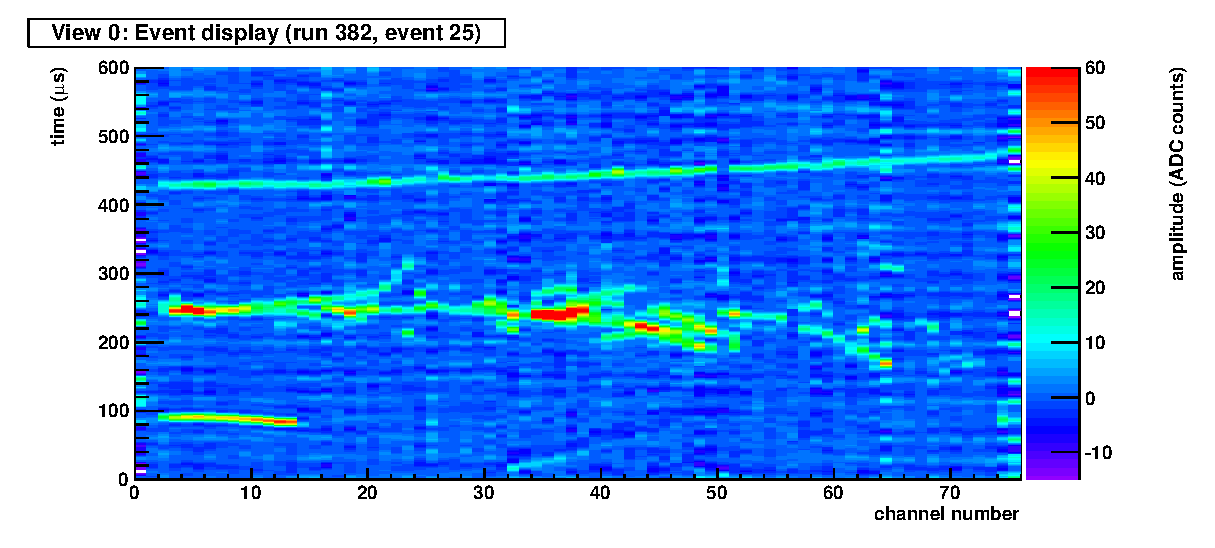
\includegraphics[width=100mm]{fig/Textbook.eps}
 \end{center}
 \caption{Event display of 800 MeV/$c$ electron triggered event.
Accidentally overlapped with a proton and a pion.}
 \label{Fig:Textbook}
\end{figure}

\begin{figure}[htbp]
 \begin{center}
  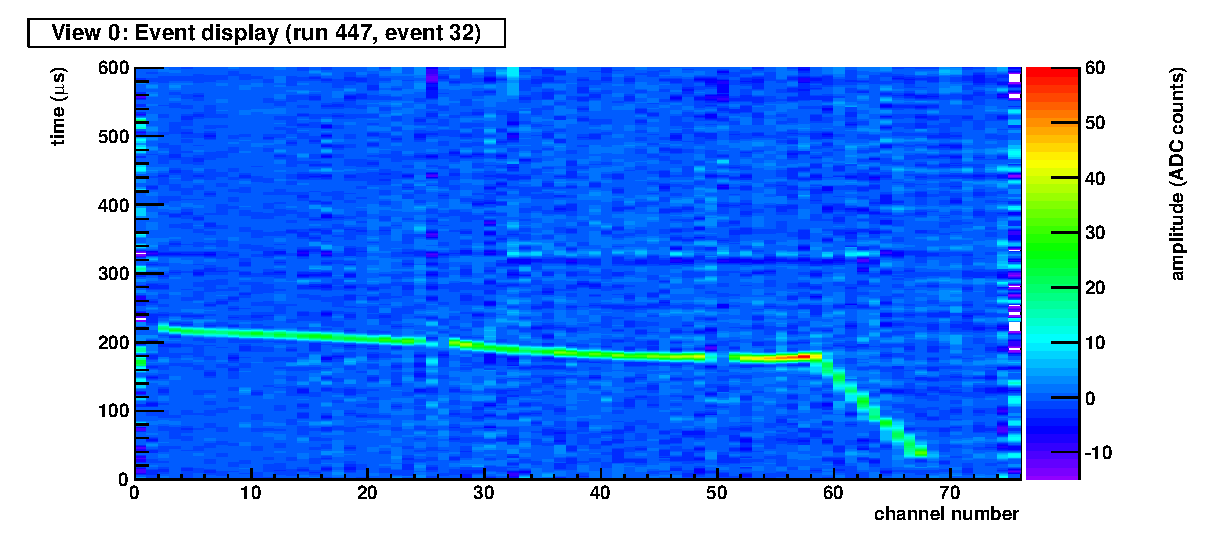
\includegraphics[width=100mm]{fig/Kmunu.eps}
 \end{center}
 \caption{Event display of Kaon 630 MeV/$c$ triggered event}
 \label{Fig:Kmunu}
\end{figure}

%\subsection{Beam Quality}
\subsection{Beam Quality(Purity)}

We have several beam counters to indentify beam particles event by event(see Fig\ref{fig:Beamline}).Using this when taking data, we can get data of interest selectively.The following describe how to identify beam particles with the typical data including $K^{+}$, $\pi~{+}$, $e^{+}$, $p$ events, which have the momentum adjusted $\sim$800MeV/c.\\

\begin{figure}[htbp]
  \centering
  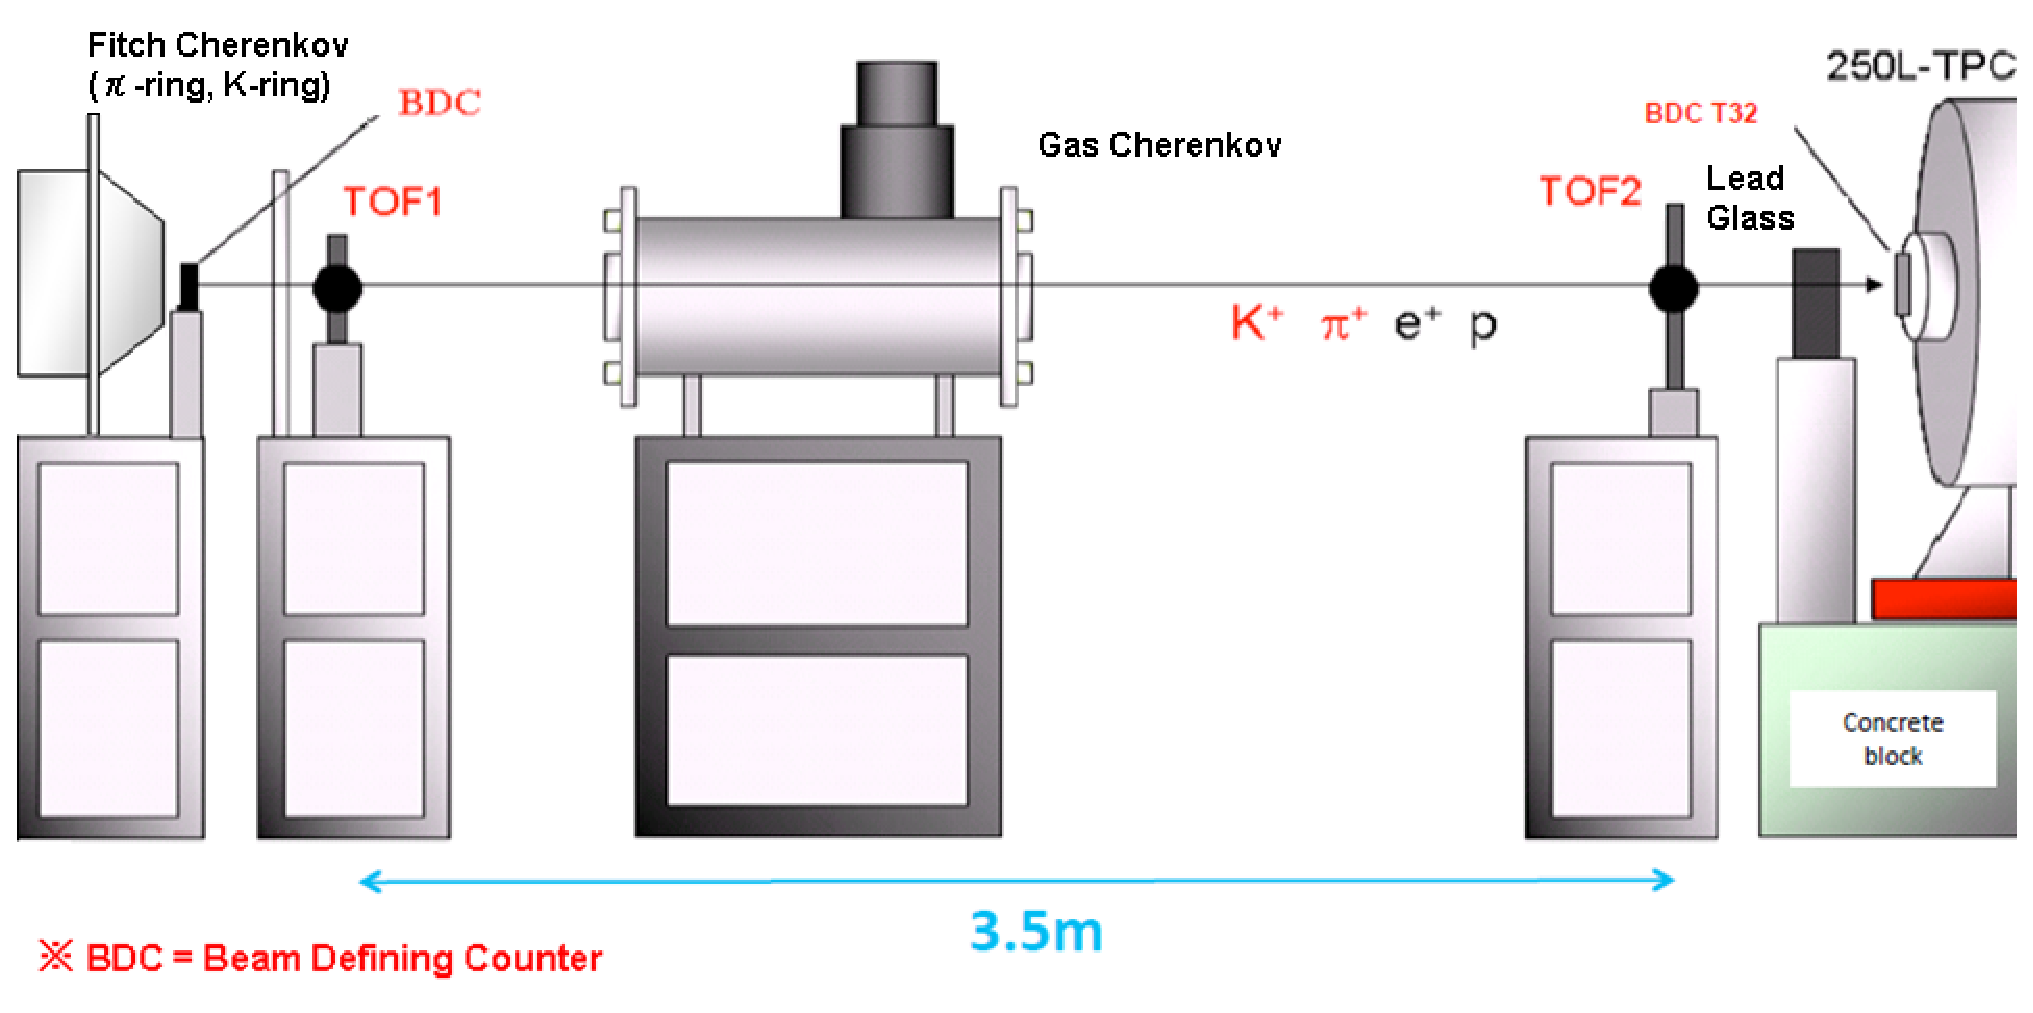
\includegraphics[width=10cm,clip]{fig/Beamline.eps}
  \caption{Instruments on K1.1BR Beam Line}
  \label{fig:Beamline}
\end{figure}

Leaded particles to K1.1BR beamline pass the Fitch Cheernkov Counter at first.
Fitch Cherenkov Counter can select particles with diffrerences of angle of cherenkov light which they radiate.
Fifure\ref{fig:FC_KPI} shows the respose of the Fitch Cherenkov Counter.
The horizontal axis shows the total amount of PMT signal where cherenkov light of 800MeV/c $\pi$ can be detected.
The vertical axis shows that of 800MeV/c $K$.
Signals are distinctly seperated to three cluster and can be categolized as following.\\

\begin{enumerate}
\item FC Signal($\pi$)$<$1450 \& FC Signal($K$)$>$2000 \\
\item FC Signal($\pi$)$<$1450 \& FC Signal($K$)$<$2000 \\
\item FC Signal($\pi$)$>$1450 \& FC Signal($K$)$<$2000 \\
\end{enumerate}

Appearently, particles within the region 1 are $K^{+}$ candidates.
Particles within region 2 are $p$ candidates because 800MeV/c $p$ is impossible to radiate cherenkov light.
Particles within region 3 are $\pi^{+}$ or $e^{+}$ candidates because their angle of cherenkov light are almost same level.\\

\begin{figure}[htbp]
  \centering
  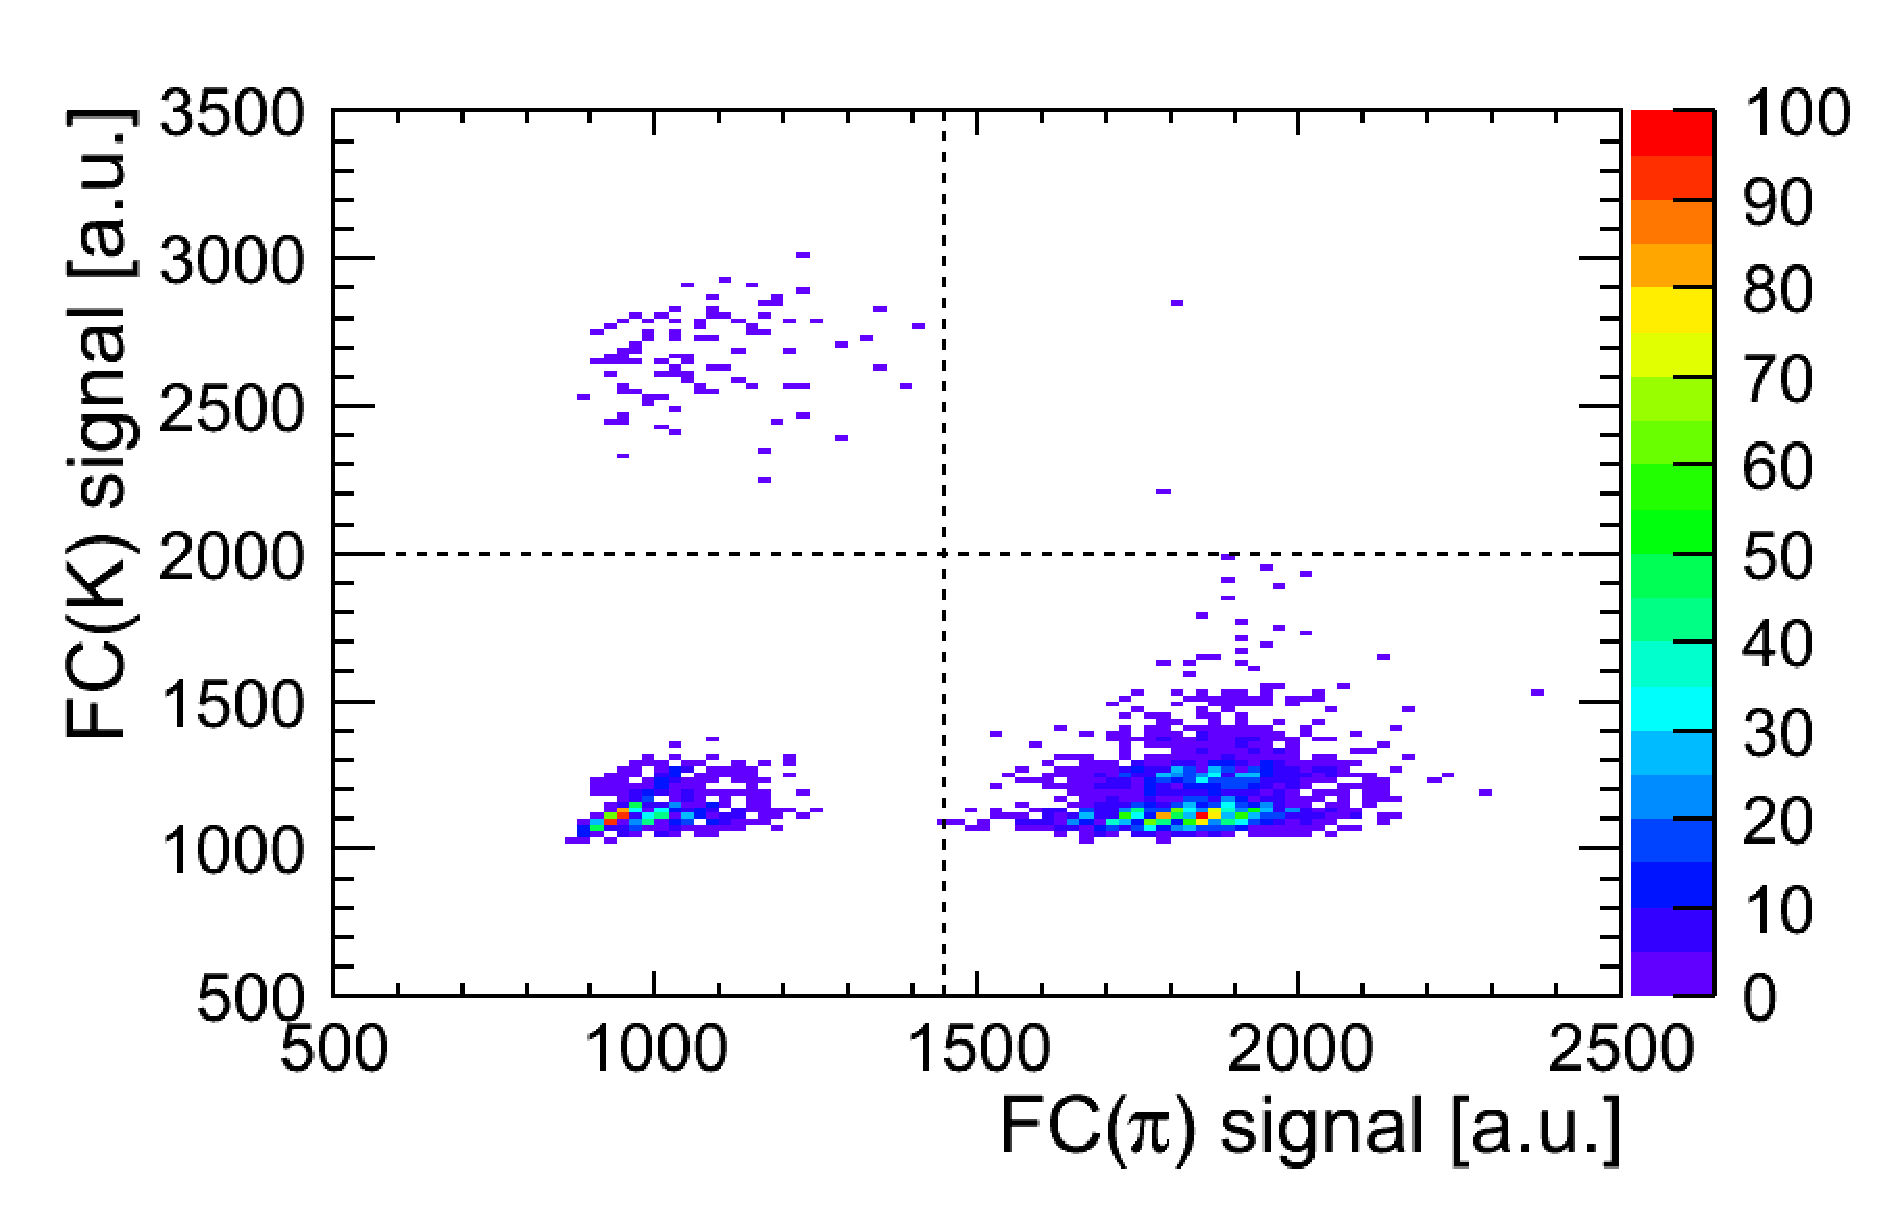
\includegraphics[width=10cm,clip]{fig/FC_KPI.eps}
  \caption{Fitch Cherenkov Counter}
  \label{fig:FC_KPI}
\end{figure}

Gas Cherenkov Counter can select $e^{+}$ from the other particles because only $e~{+}$ can radiate cherenkov light at the refractive index of this gas.
Figure\ref{fig:GC} shows the responce of the Gas Cherenkov Counter.
The horizontal axis shows the PMT signal of the Gas Cherenkov Counter.
The vertical axis shows the number of events.
Fitting the pedestal with gaussian function,
the events larger than the value added $\sim$3.5$\sigma$ to the mean of the pedestal is $e^{+}$ candidates.In this case, GC signal is required more than 104.7 to be $e^{+}$ candidates.\\

\begin{figure}[htbp]
  \centering
  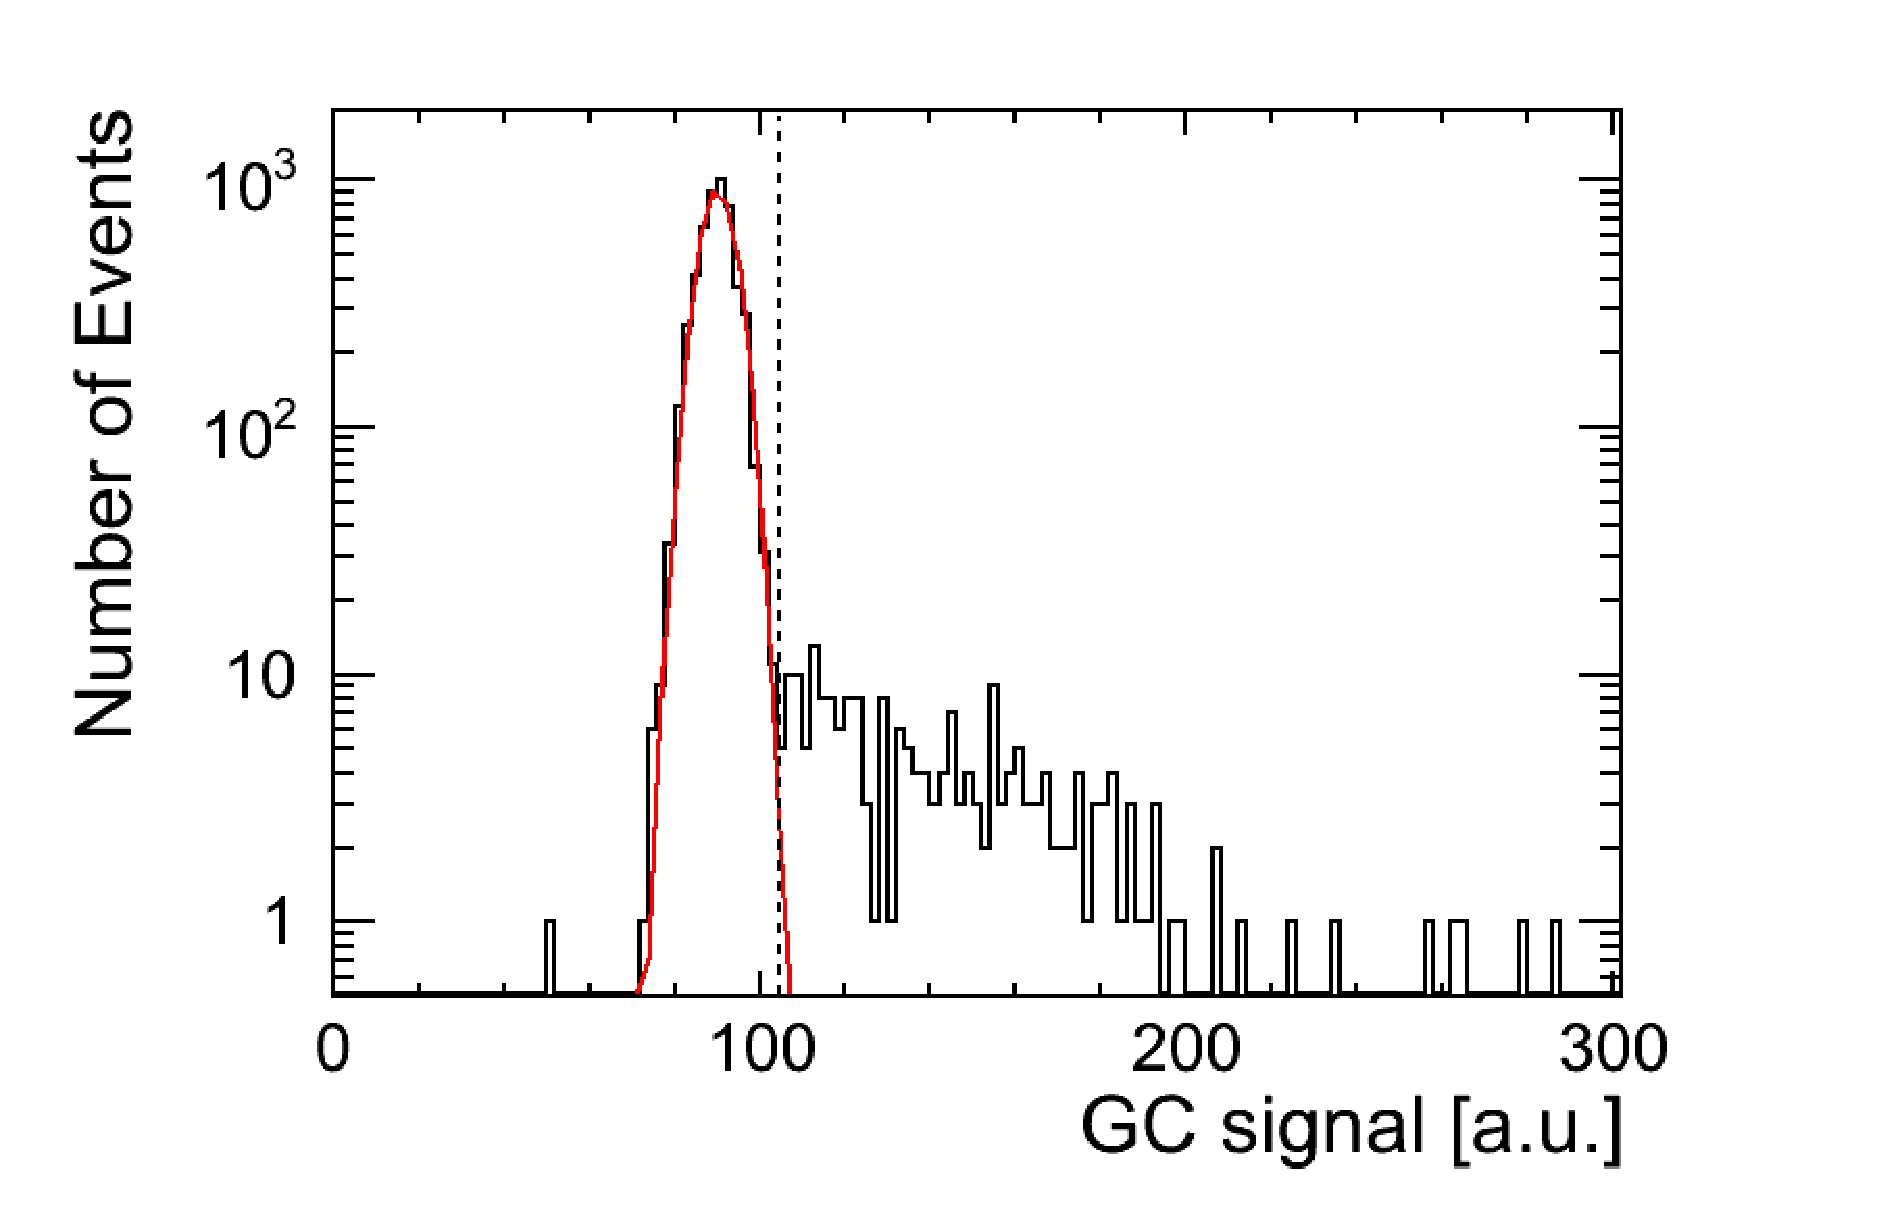
\includegraphics[width=10cm,clip]{fig/GC.eps}
  \caption{Gas Cherenkov Counter}
  \label{fig:GC}
\end{figure}

There are two TOF Counters which has $\sim$200ps resolution 3.5m apart, 
and each particle can be selected with the difference of time of flight between them.
Following table\ref{tb:TOF_expect} is calcurated time of flight when each 800MeV/c particle passes two conters.
As this table shows, $e~{+}$ and $\pi^{+}$ cannot selected because the difference of time of flight is too short for the TOF resolution.\\

\begin{table}
  \centering
  \begin{tabular}[htb]{c|cccc}\hline
    particle & $e^{+}$ & $\pi^{+}$ & $K^{+}$ & $p$ \\ \hline
    Mass(MeV) & 0.511 & 139.57 & 493.68 & 938.27 \\
    Time of Flight($ns$) & 11.67 & 11.84 & 13.71 & 17.98 \\ \hline
  \end{tabular}
  \caption{Time of flight of eash particle}
  \label{tb:TOF_expect}
\end{table}

Figure\ref{fig:TOF} shows responce of the TOF Counters.
The horizontal axis shows the time of flight between TOF1 and TOF2 Counter.
The vertical axis shows the number of events.
Signals have clearly divided three structures.
From table\ref{tb:TOF_expect}, in asending order of time of flight the first structure include $e^{+}$ or $\pi^{+}$ candidates,
and the second struature include $K^{+}$ candidates,
and the third structure include $p$ candidates.
The cut value to separete the first strucuture and the second structure is $\sim$4.5$\sigma$ (in this case, the value is setted 13.15ns), and because the second structure and the third structure is clearly separated, the cut value to select them is setted 16.47ns fully apart from the second structure.\\

\begin{figure}[htbp]
  \centering
  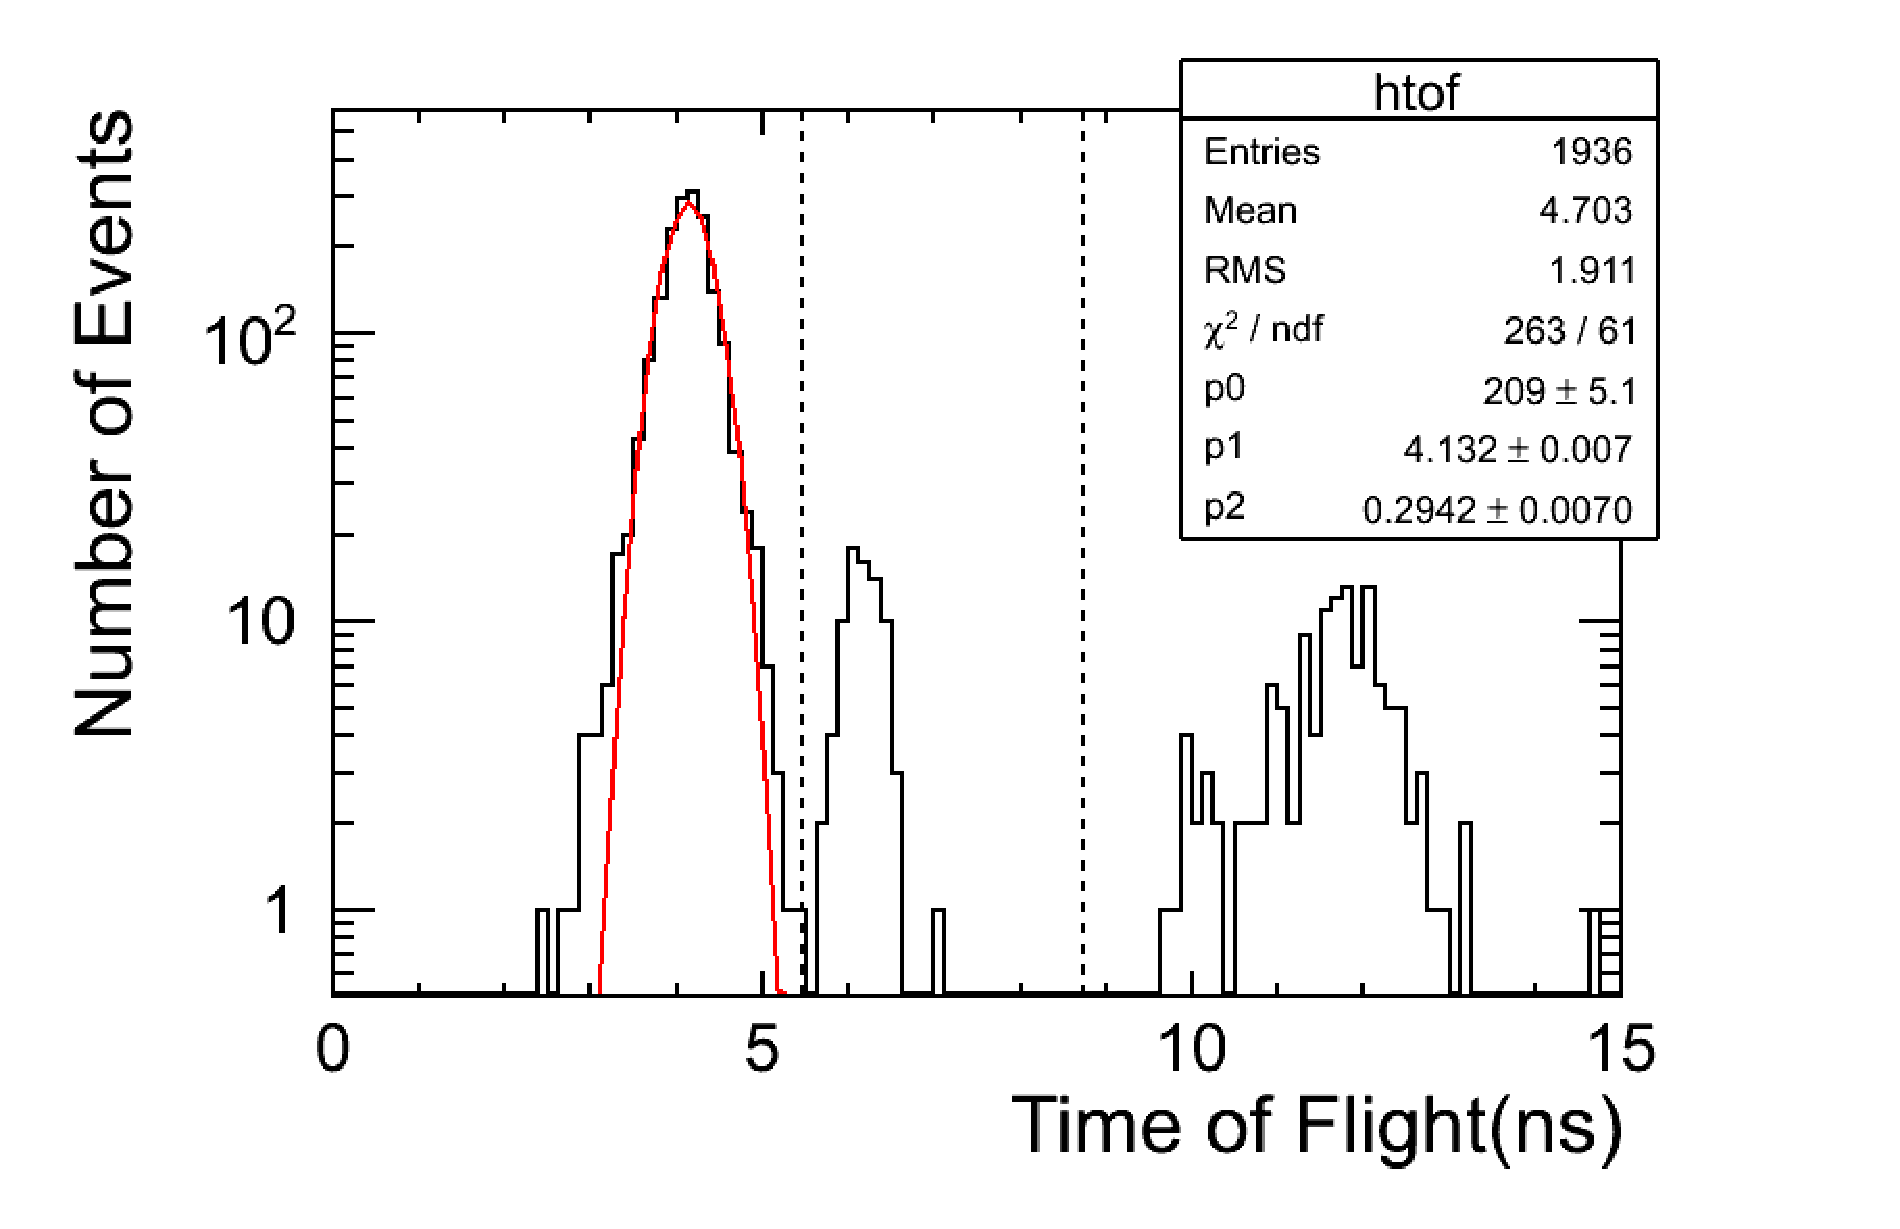
\includegraphics[width=10cm,clip]{fig/TOF.eps}
  \caption{TOF Counter}
  \label{fig:TOF}
\end{figure}

$K^{+}$ can selected very efficiently with Fitch Cherenkov Counter,
so we require the condition FC Signal($K$) is more than 2000
to get the date of $K$ in taking data.
Figure\ref{fig:TOF_cut} shows responce of the TOF Counters before and after above cut.
The histgram which filled with black is what is after cut.
This figure shows we can get high-purity $K^{+}$ samples with this condition.

\begin{figure}[htbp]
  \centering
  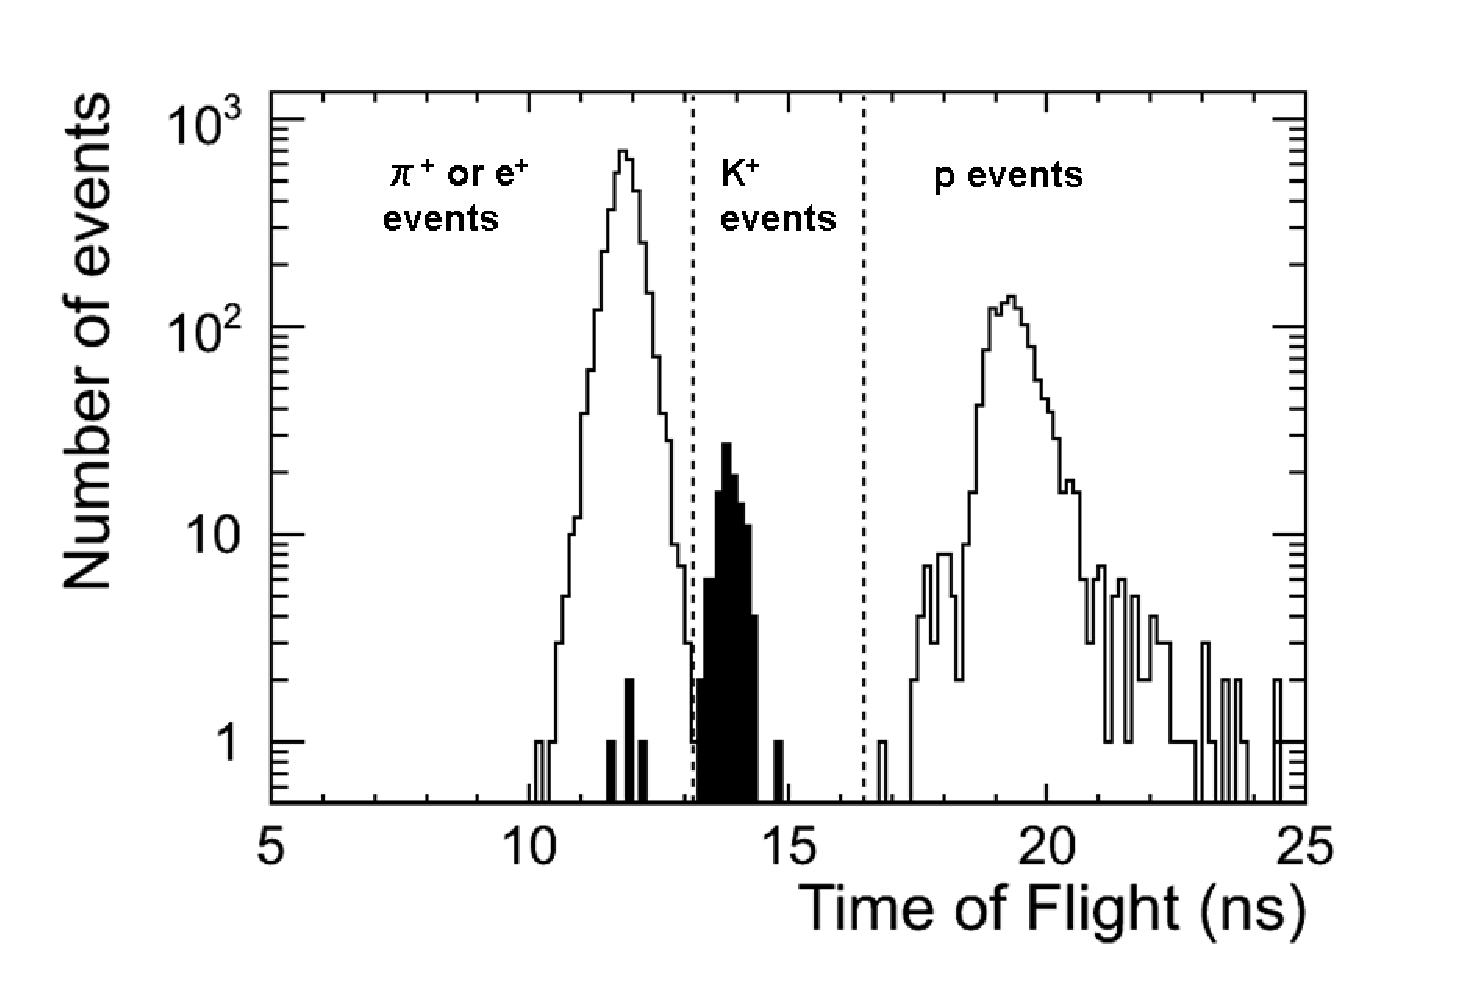
\includegraphics[width=10cm,clip]{fig/TOF_cut.eps}
  \caption{TOF Counter}
  \label{fig:TOF_cut}
\end{figure}

Particles which satisfy all conditions for the same candidate are identified themselves, and the others are defined `uncertain` particles.
Herewith, we can identify beam particles with high purity before injection to 250L detector.
Table\ref{tb:component} shows the beam components of the data used for analysis.\\

\begin{table}
  \centering
  \begin{tabular}[htb]{ccccccc}\hline
    Run Number    & $e^{+}$ & $\pi^{+}$ & $K^{+}$ & $p$   & $uncertain$ & Number of Events \\ \hline
    42            & 68      & 1617      & 27      & 232   & 5           & 1949             \\
    48            & 128     & 1594      & 78      & 126   & 11          & 1937             \\
    49            & 0       & 341       & 0       & 1146  & 12          & 1499             \\
    52            & 0       & 1         & 3126    & 0     & 76          & 3203             \\
    55            & 0       & 6         & 8386    & 0     & 208         & 8600             \\
    59            & 0       & 8         & 5863    & 0     & 119         & 5963             \\
    60            & 0       & 1         & 1870    & 0     & 40          & 1911             \\ \hline
  \end{tabular}
  \label{tb:component}
  \caption{Beam components of data ued for analysis}
\end{table}

Run 52,55,59 and 60 are the data required the condition FC Signal($K$) is more than 2000 in taking data.
As table\ref{tb:component} shows, these data is almost occupied $K^{+}$ events and the ratio is $\sim$98\% on average.

 
%\subsection{Beam Energy, Position}
   \section{Beam Energy, Position}
   \subsection{Beam Energy}
 
   30GeV proton beam hits to target T1 in Hadron hall.
   It generates many particles like kaon, pion, muon, electron, and
   so on.
   We take the particles that has 800MeV/c momentum from this beam by
   using D1 magnet.\\
   \ \ For this analysis, a beam momentum at BDC after passing through the
   K1.1Br beam line is required.
   We estimate a beam momentum using simple MC simulation.
   Figure \ref{K11Br_Beam_line} shows MC simulation's geometory.
   This time, beam line is straight and has no electric and magnetic
   field.
   MC simulation shoot 800MeV/c kaon and pion as pencil beam.

   Figure \ref{k_pi_momentum} shows kaon and pion momentum distribution
   using this MC simulation.
   Actually, kaon momentum distribution peak is adjusted so that kaon
   decay point of MC simulation is consistent with data.
   Section \ref{kaon_energy_section} explains this point.
   And proton momentum is estimated in other way, using TREK detector
   TOF information.
   Section \ref{proton_energy_section} shows proton momentum distribution.

   \subsubsection{Kaon energy}\label{kaon_energy_section}

We adjust momentum peak of figure ?? and set Kaon beam energy  the point that the decay points of Kaon in data and simulation are good agreement. The distribution of decay poins are plotted in Figure\ref{DecayPoint_hough}.
\begin{figure}[!htb]
  \begin{center}
    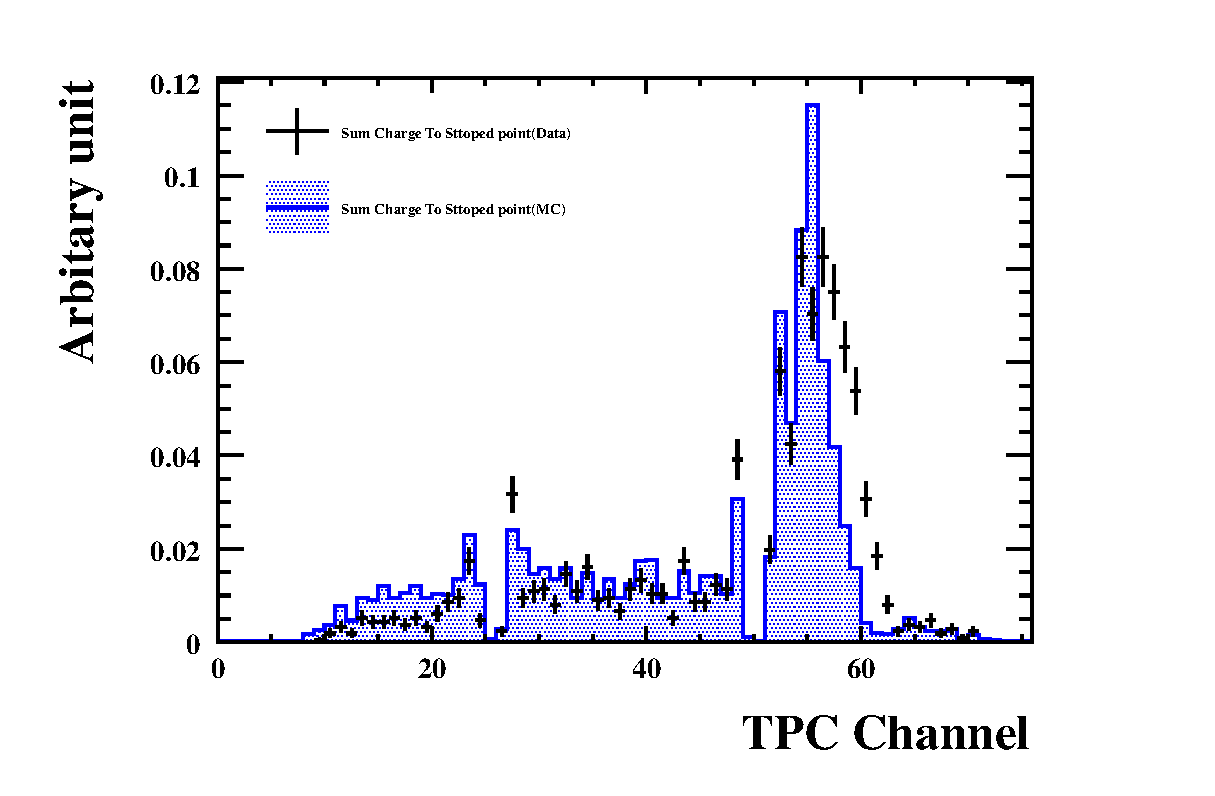
\includegraphics[width=70mm]{fig/cdp_hough.eps}
  \end{center}
  \caption{Decay point distribution of Data and MC}
  \label{DecayPoint_hough}
\end{figure}

   \subsubsection{Proton energy}\label{proton_energy_section}
   asuka




   \subsection{Energy deposition in degrader}
   Because of having high energy, kaon beam from BDC passes through 250LAr TPC.
   So that kaon stops in 250LAr TPC, we put degrader, which reduce
   beam energy, on beam line.
   In this experiment, we used lead glass and lead block as degrader.
   We estimate energy deposition in degrader by using MC simulation.
   Figure \ref{energy_deposition} shows energy deposition in degrader.
   
   \subsection{Beam Position}
   Before taking data, we measured a beam profile on the front of
   250LAr TPC by using plastic scintillation counter.
   Figure \ref{beamprofile_250L} shows beam profile on the front of
   250LAr TPC.

   \begin{figure}[!htb]
    \centering
    \centering
    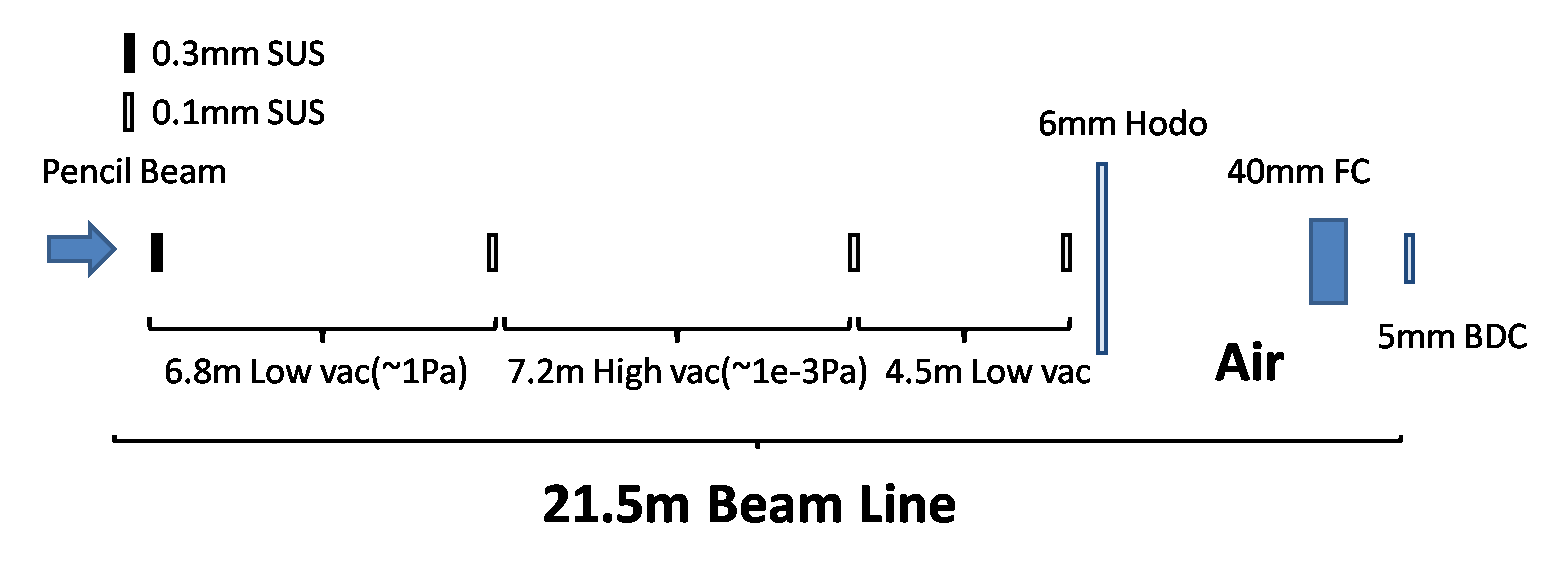
\includegraphics[width=11cm,clip]{./fig/K11Br_beamline_sim.eps}
    \caption{K1.1 Br beamline}
    \label{K11Br_Beam_line}
   \end{figure}



   \begin{figure}[!htb]
    \centering
    \centering
    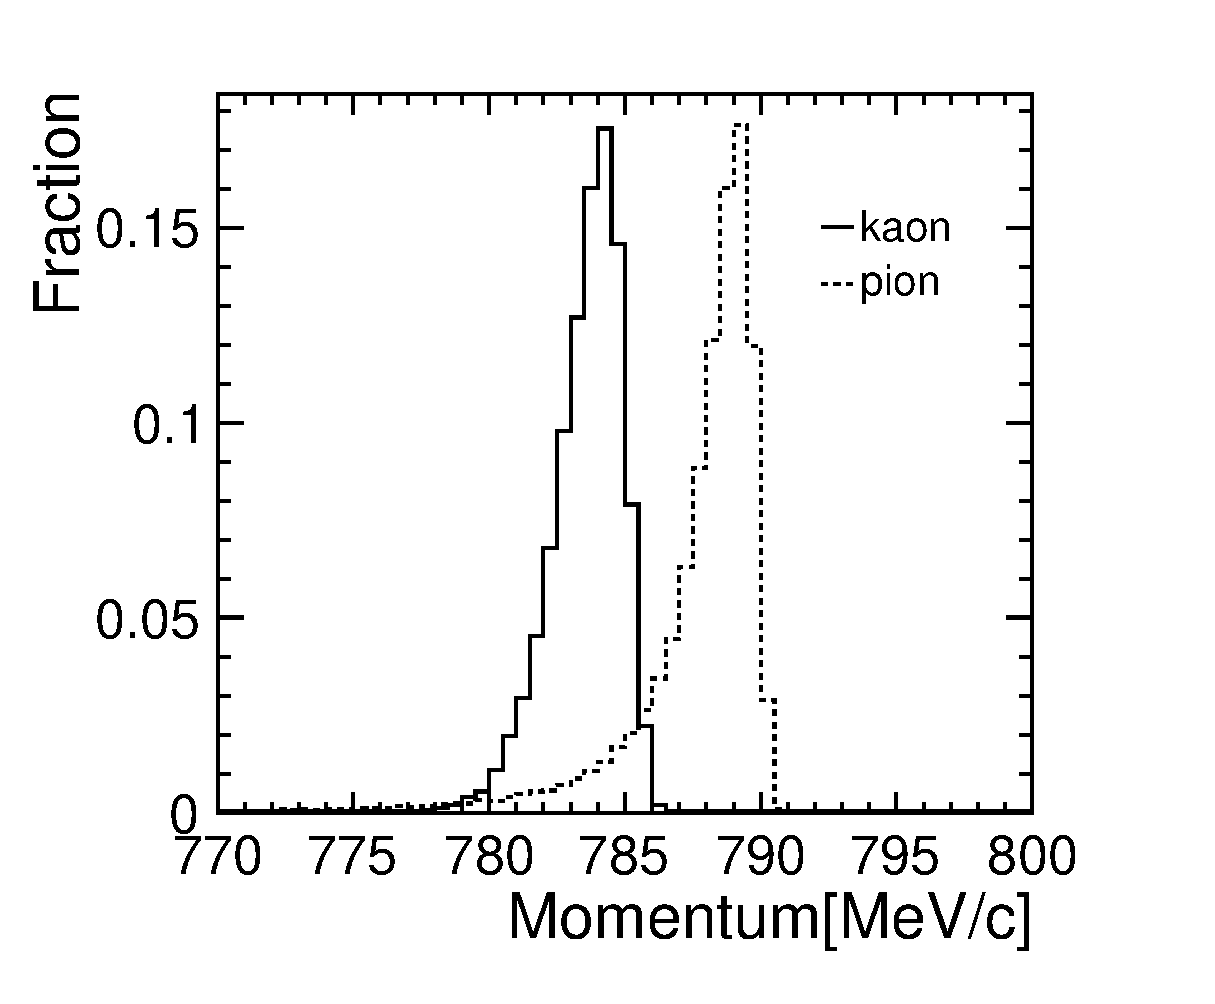
\includegraphics[width=11cm,clip]{./fig/Kaon_pion_momentum_nogrid.eps}
    \caption{kaon and pion momentum distribution at BDC}
    \label{k_pi_momentum}
   \end{figure}


   \begin{figure}[!htb]
    \centering
    \centering
    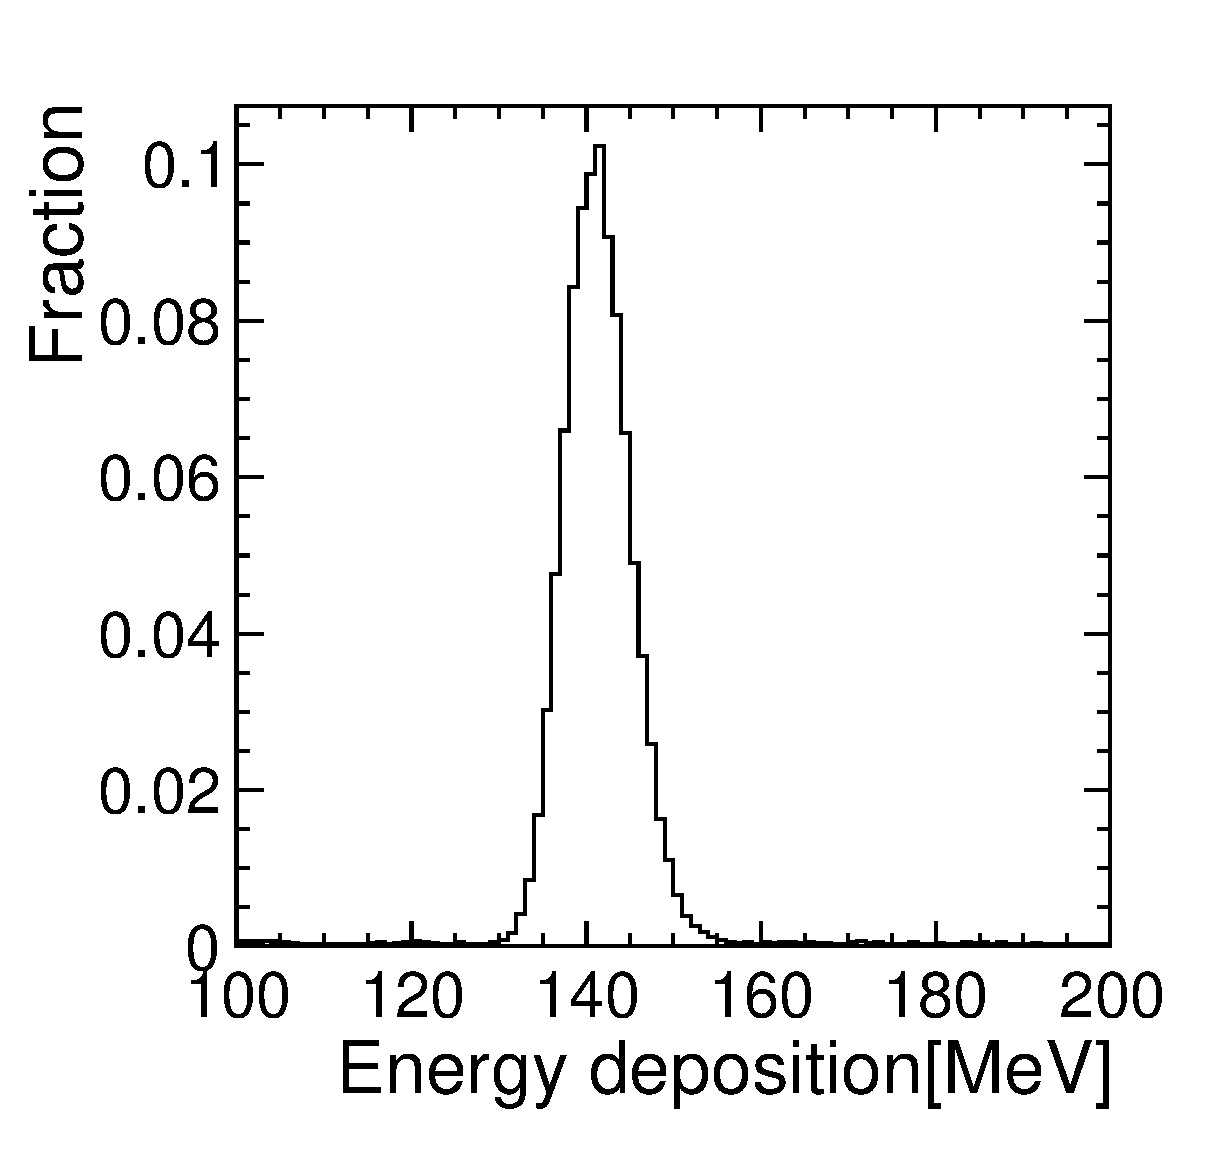
\includegraphics[width=11cm,clip]{./fig/energy_deposition.eps}
    \caption{energy deposition in degrader}
    \label{energy_deposition}
   \end{figure}


   \begin{figure}[!htb]
    \centering
    \centering
    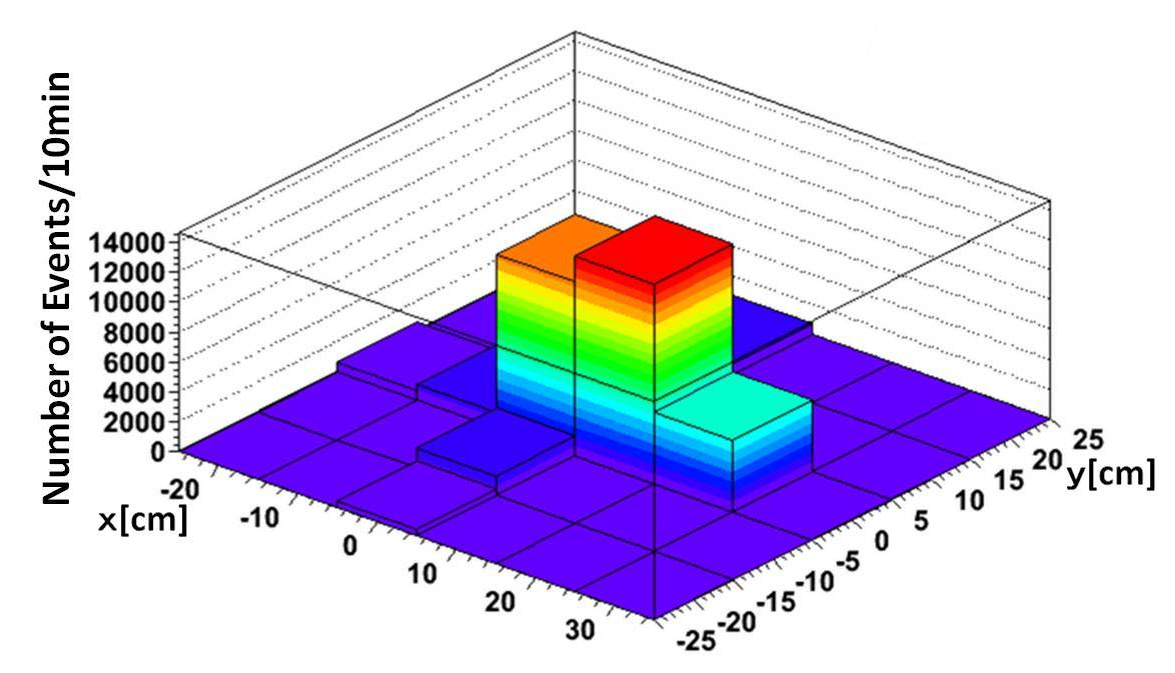
\includegraphics[width=11cm,clip]{./fig/BeamProfile3.eps}
    \caption{Beam profile on the front of 250LAr TPC}
    \label{beamprofile_250L}
   \end{figure}


%%%%%%%%%%%%%%%%%%%%%%%%%%%%%%%%%%%%%%%%%%%%%%%%%%
%\section{Software Framework}
%%%%%%%%%%%%%%%%%%%%%%%%%%%%%%%%%%%%%%%%%%%%%%%%%%
%%%%%%%%%%%%%%%%%%%%%%%%%%%%%%%%%%%%%%%%%%%%%%%%%%
\section{Software Framework}
%%%%%%%%%%%%%%%%%%%%%%%%%%%%%%%%%%%%%%%%%%%%%%%%%%
Qscan is a general purpose software package for LArTPC analysis(reference)
which provides,
\begin{itemize}
\item event reconstruction:  noise reduction, hit finding, clustering, and tracking...
\item event simulation: GEANT VMC with ROOT geometry, ionization electron recombination, drift, digitization... 
\item event visualization: display raw data waveform and reconstructed quantities
\end{itemize}

%%%%%%%%%%%%%%%%%%%%%%%%%%%%%%%%%%%%%%%%%%%%%%%%%%
%\section{Event Reconstruction}
%%%%%%%%%%%%%%%%%%%%%%%%%%%%%%%%%%%%%%%%%%%%%%%%%%
%%%%%%%%%%%%%%%%%%%%%%%%%%%%%%%%%%%%%%%%%%%%%%%%%%
\section{Event Reconstruction}
%%%%%%%%%%%%%%%%%%%%%%%%%%%%%%%%%%%%%%%%%%%%%%%%%%
\subsection{Noise Reduction}

Figure \ref{Fig:beforeFFT} shows raw waveform of the TPC signal
before applying any noise reduction. Two waveforms shown in this plot
are channel 13 and 37 in Figure~\ref{Fig:Textbook} which are roughly
proton stopped point and electron shower maximum point, respectively.
Signal-to-noise ratio for this particular case is poor and pion signal 
which is supposed to be t=400 $\mu$s is almost hidden by the noise. 
While time width of TPC signal is few $\mu$s which is determined by
drift time between anode and anode-grid, dominant noise component looks
higher frequency. To reduce such noises, we have applied FFT 
(Fast Flourier Transformation) filter to cut the high frequency component.
Figure \ref{Fig:FFT} shows amplitude as a function of frequency
for the same event. This clearly shows dominant noise component with
$>$ 200 kHz has good separation with signal component ($<$ 100 kHz).
Figure \ref{Fig:afterFFT} shows the waveform after removing high frequency
($>$ 80 kHz) component by the FFT filter. Signal-to-noise ratio is dramatically
improved. On the other hand, we expect certain bias to the signal charge
measurement by this filter, and it will be discussed in Section x.

\begin{figure}[htbp]
 \begin{center}
  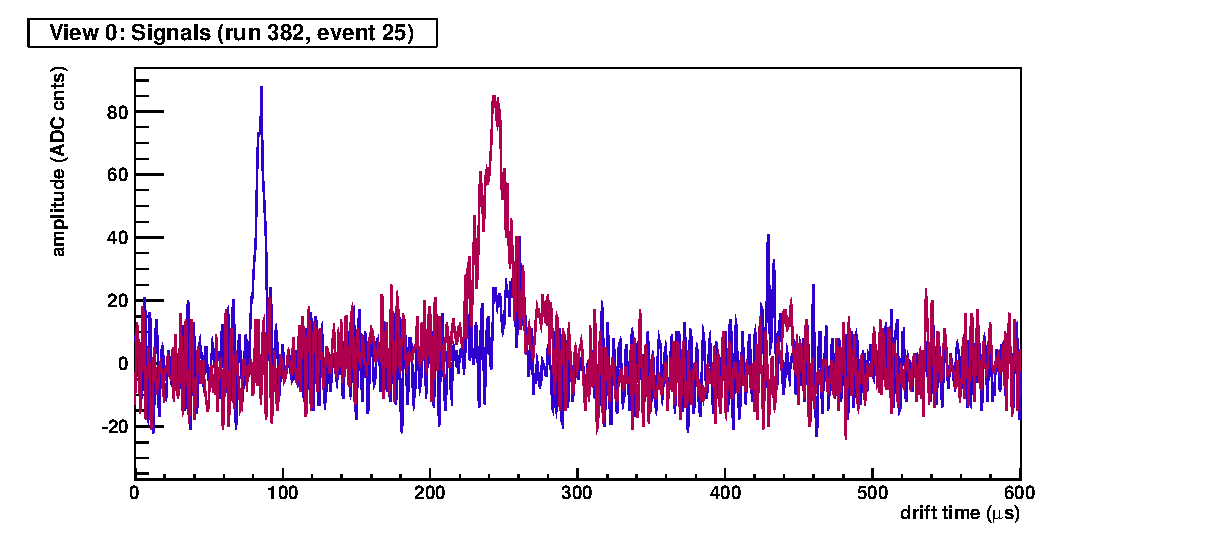
\includegraphics[width=100mm]{fig/beforeFFT.eps}
 \end{center}
 \caption{TPC raw signal waveform for "Textbook" event channel 13 and 37.}
 \label{Fig:beforeFFT}
\end{figure}

\begin{figure}[htbp]
 \begin{center}
  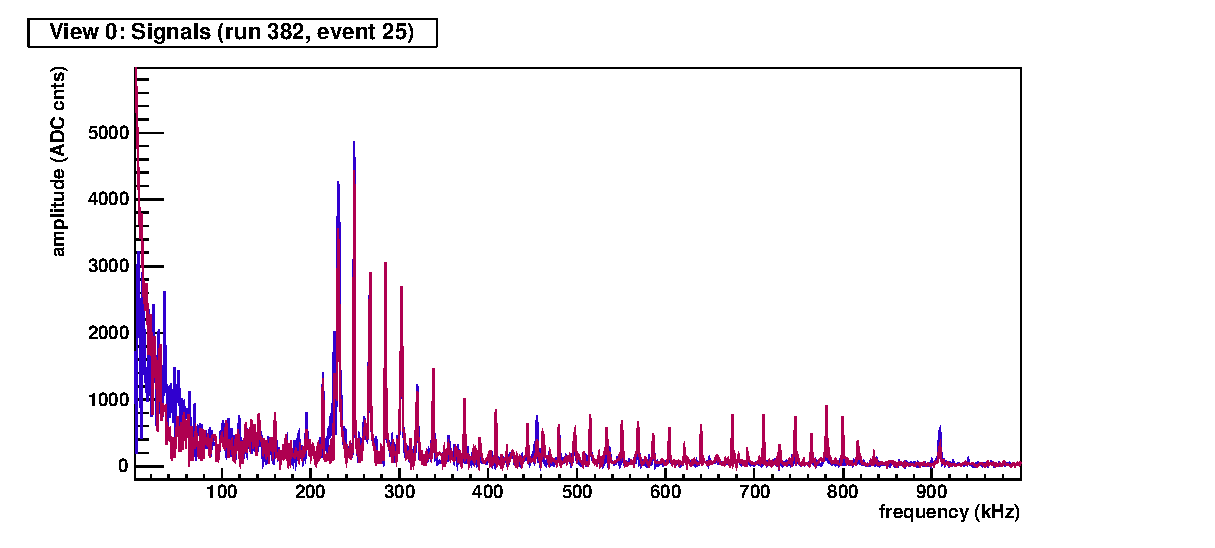
\includegraphics[width=100mm]{fig/FFT.eps}
 \end{center}
 \caption{FFT frequency amplitude distribution}
 \label{Fig:beforeFFT}
\end{figure}

\begin{figure}[htbp]
 \begin{center}
  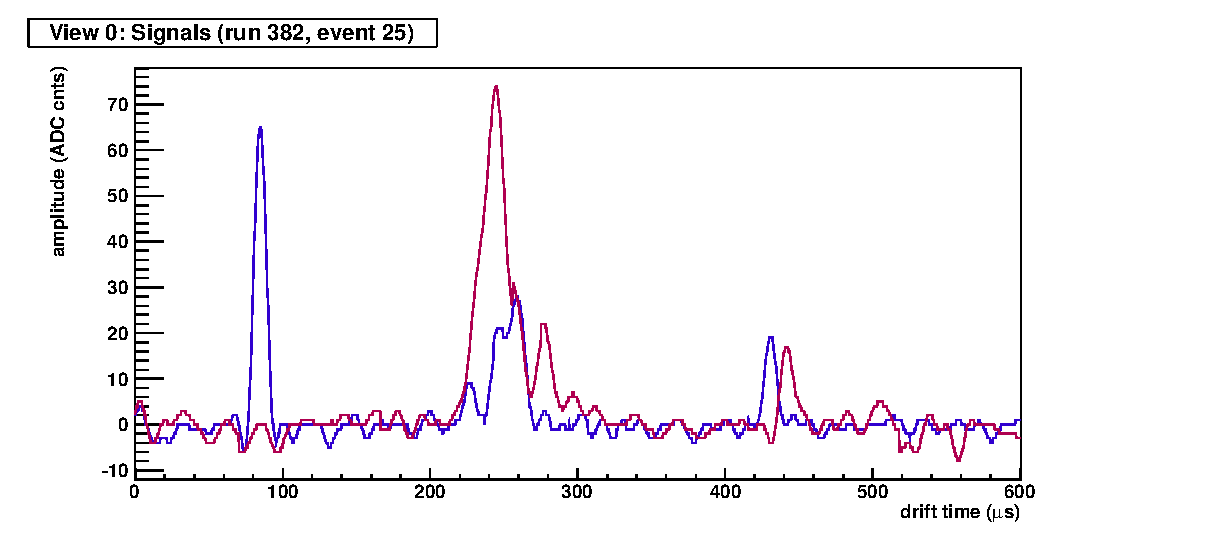
\includegraphics[width=100mm]{fig/afterFFT.eps}
 \end{center}
 \caption{TPC signal waveform after cutting the frequency $>$ 80 kHz.}
 \label{Fig:afterFFT}
\end{figure}


%\subsection{Hit Finding/Clustering}
\subsection{Hit Finding/Clustering}
After noise reduction we find signal hits and create clusters associated to single tracks. 
Hit is defined as bump over given threshold in a channel. 
After finding all hits in an event, we construct cluster by merging adjacent hits. 
The example of hit finding and clustering is shown in Fig~\ref{fig:Clustering}, which indicates reasonable hit and cluster findings. 
Threshold of hit finding is 6 ADC counts, which is about 2.5$\sigma$ from typical data noise level (as shown in Fig~\ref{Fig:beforeFFT}) and keeping more than 99\% of Kaon hit finding efficiency from simulation.
% noise level from outside window of PhysicsOct55 (rms~2.49)
ADC count distribution is fitted by step funcion plus Gaussian to estimate the charge of hit in ADC $\times$ $\mu$s unit.
Fitting $\chi^2 < 3$ and $2.5<$~(time~width~of~hit)~$<8$~$\mu$s are required to remove noise hits further.

\begin{figure}[htbp]
 \begin{center}
  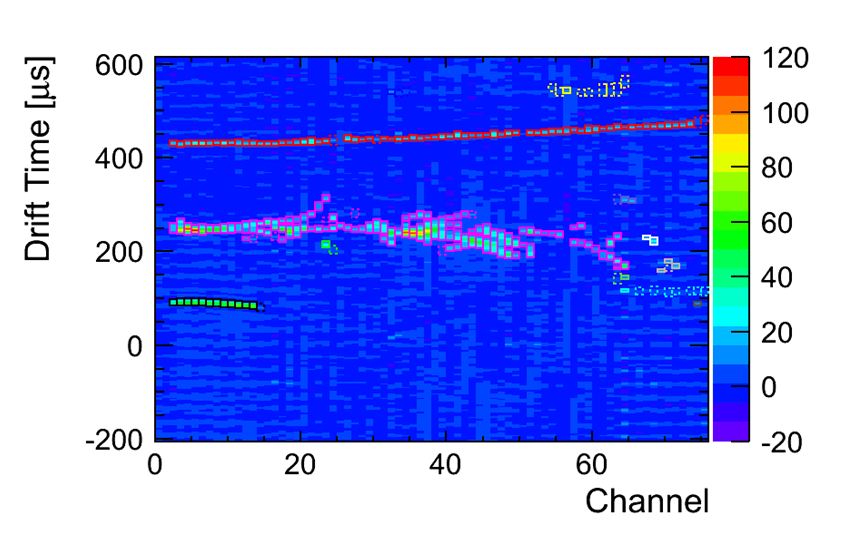
\includegraphics[width=100mm]{fig/clustering.eps}
 \end{center}
 \caption{Example of hit finding and clustering. A colored box corresponds to a hit and colors represent different clusters.}
 \label{fig:Clustering}
\end{figure}

%\begin{itemize}
%\item Plot: Finding efficiency vs threshold (Naganoma): TBU
%\item Plot: Through-going pion data Q vs pion (Tanaka)
%\end{itemize}


\subsection{Stopped Point Finding}
\subsubsection{Proton}
%\subsection{Stopped Kaon}
\subsection{Stopped Kaon}
Hough transform was invented for machine analysis of bubble chamber photographs by Paul.V.C.Hough.\cite{3069654}
We find straight lines using hough method , and find Kaon stopped point from the intersection of straight lines.\\
Figure \ref{hmap2} shows hit map like a Kaon track.
One point in the X-Y space can be transformed into sinusoidal curve in the $\rho$-$\theta$ space.Figure \ref{rho_theta2} shows sinusoidal curves in all points.
And, we find the straight line associated with the largest number of points by choosing the most dense point in $\rho$-$\theta$ space.
Next , the sinusoidal curves of the hits associated with frist straight line are removed from figure \ref{rho_theta2}.
Figure \ref{rho_theta3} shows sinusoidal curves after the hits associated with frist straight line removed.
We find second straight line using the same procedure.This procedure is repeated until there are less than three points.Figure \ref{hmap_fit} shows the two straight lines found by hough transform mehotd.\\
Kaon stopped point in the liquid argon detecor defined as charge maximum point around the intersection of some lines.


\begin{figure}[!htb]
  \begin{minipage}{0.5\hsize}
    \begin{center}
      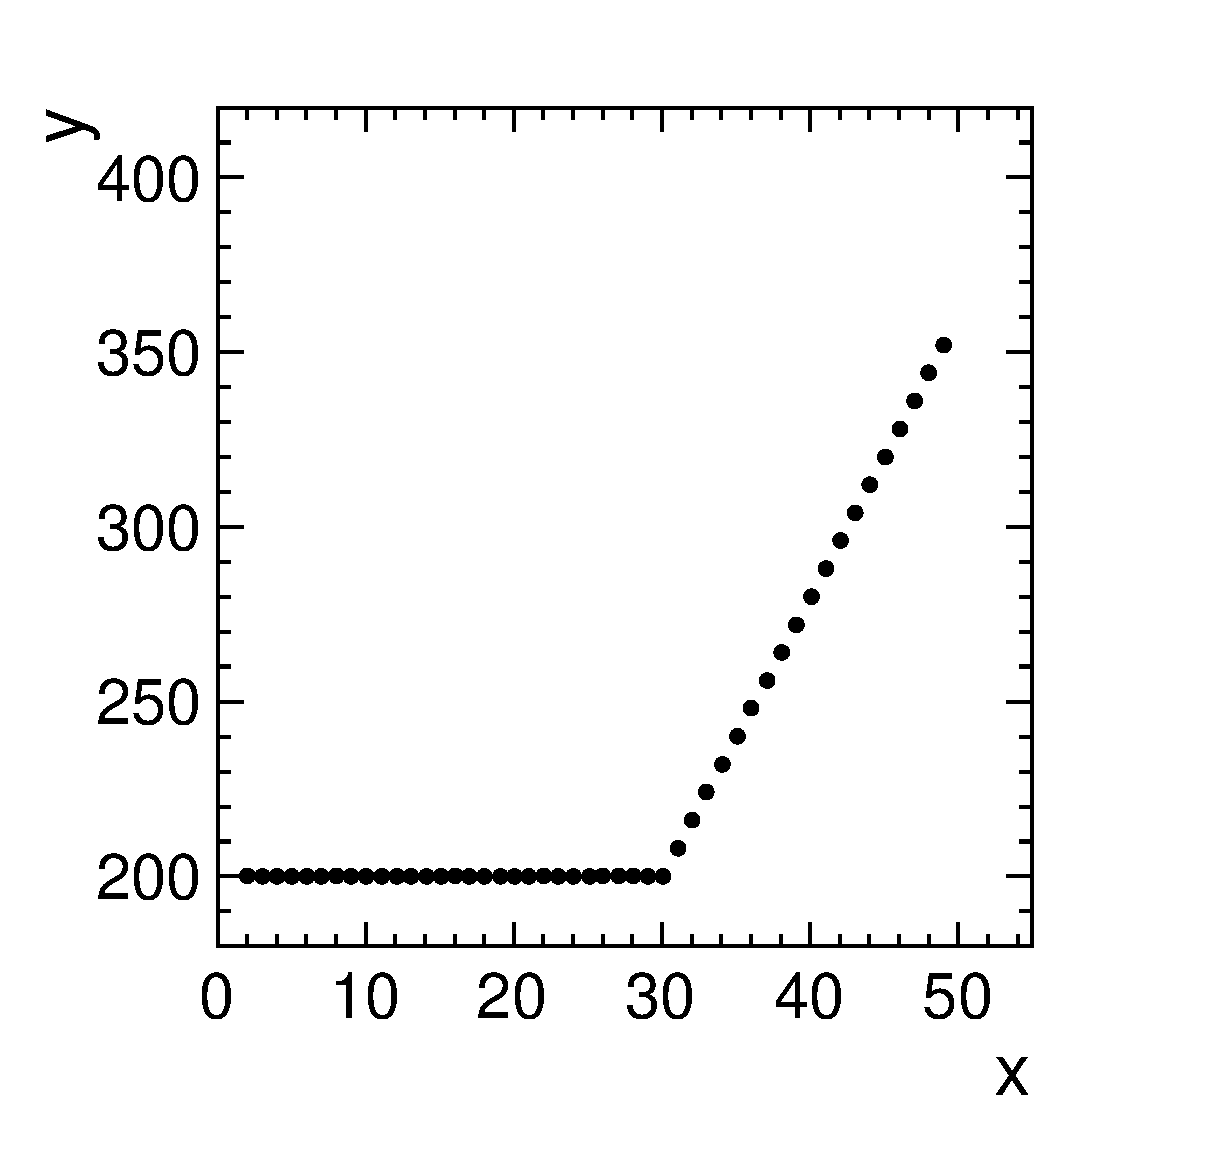
\includegraphics[width=35mm]{fig/hmap2.eps}
    \end{center}
    \caption{Hit map like a Kaon track}
    \label{hmap2}
  \end{minipage}
  \begin{minipage}{0.5\hsize}
    \begin{center}
      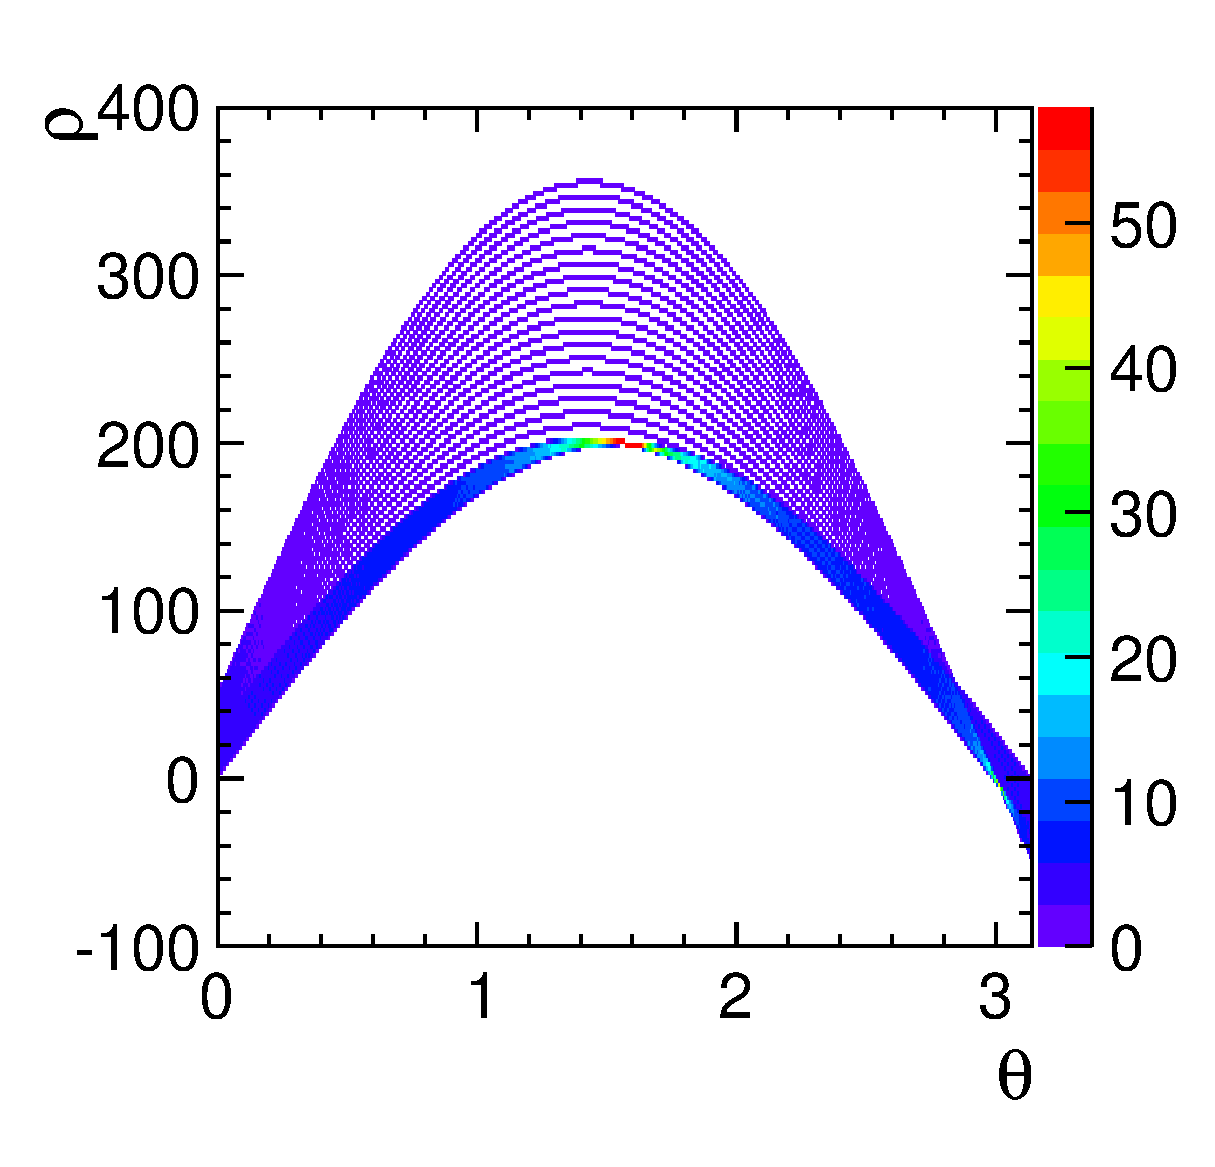
\includegraphics[width=35mm]{fig/rho_theta2.eps}
    \end{center}
    \caption{sinusoidal curves getting form all hough transformed  points of Figure \ref{hmap2}}
    \label{rho_theta2}
  \end{minipage}
  \\
  \begin{minipage}{0.5\hsize}
    \begin{center}
      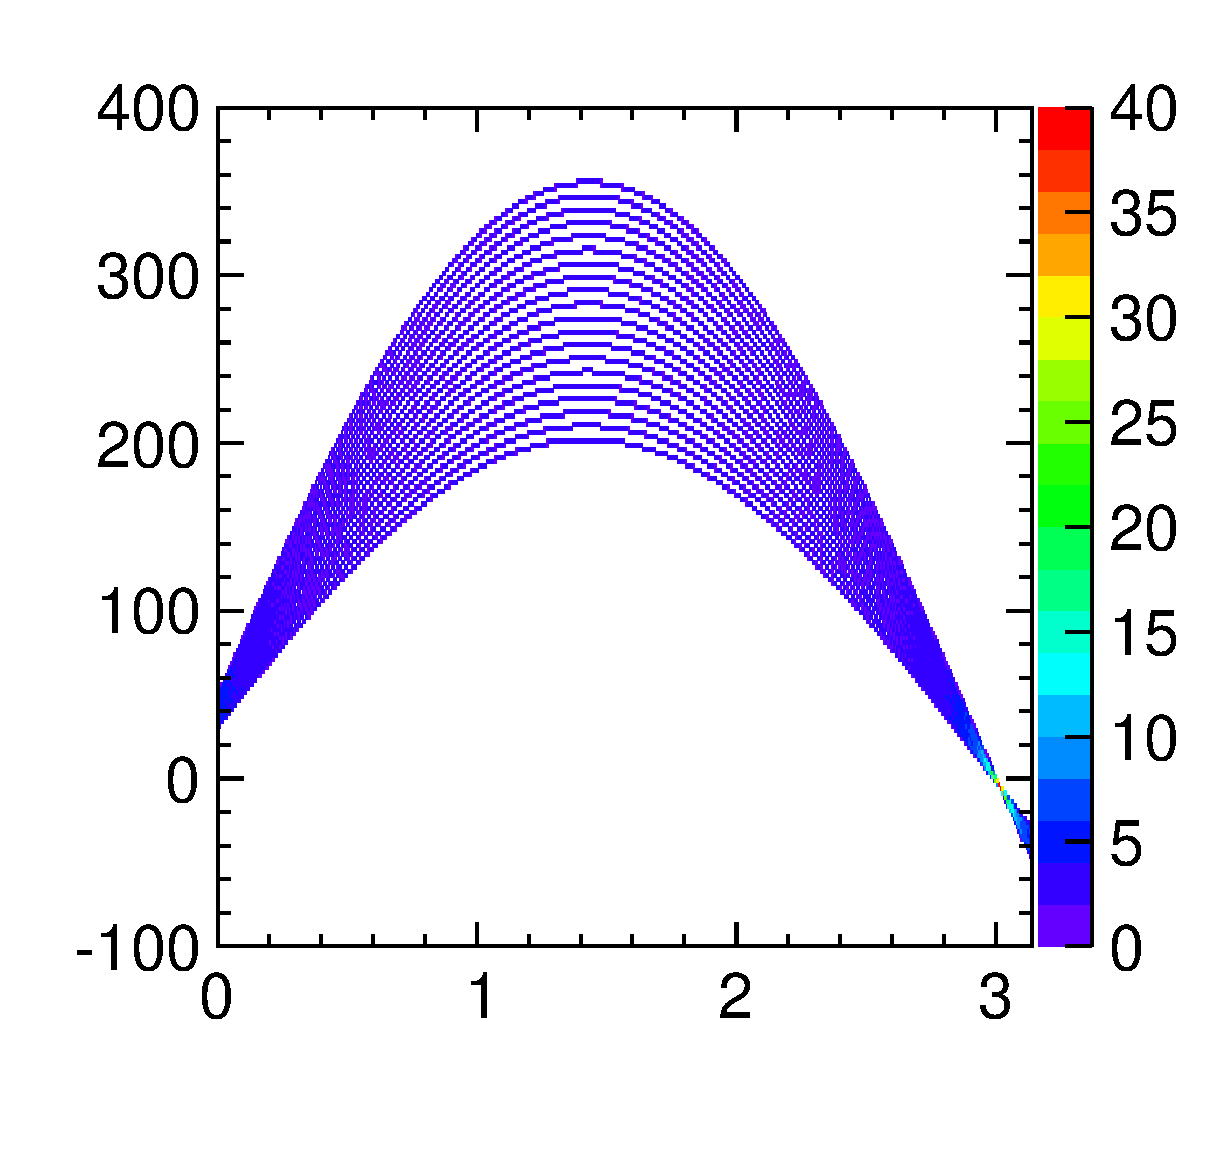
\includegraphics[width=35mm]{fig/rho_theta_kink.eps}
    \end{center}
    \caption{sinusoidal curves removed the points associated with first straight line from figure \ref{rho_theta2}}
    \label{rho_theta3}
  \end{minipage}
  \begin{minipage}{0.5\hsize}
    \begin{center}
      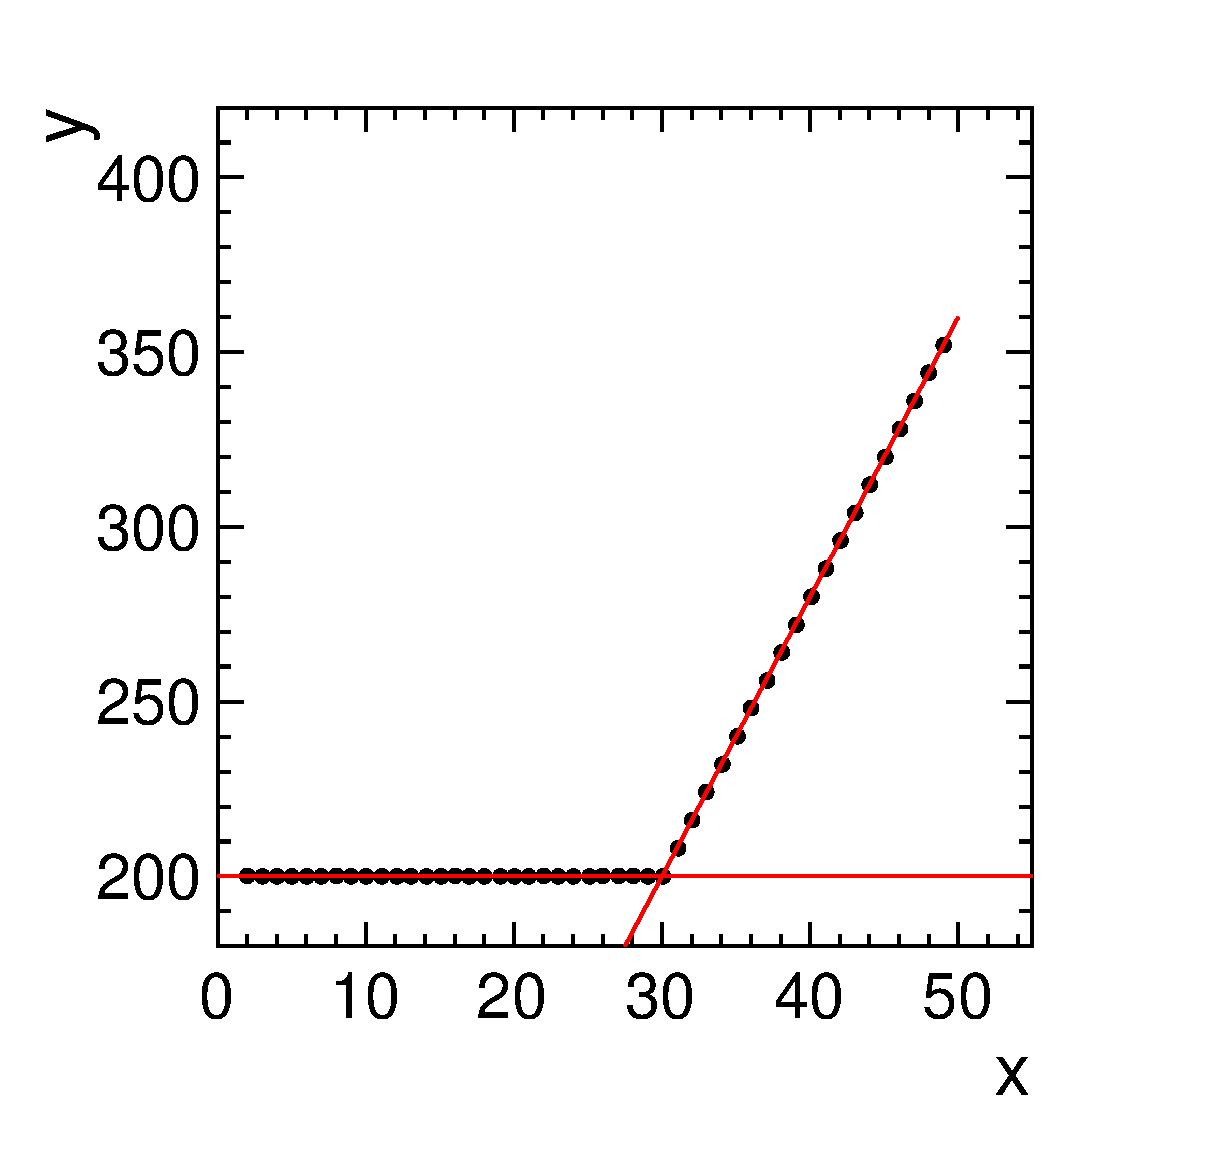
\includegraphics[width=35mm]{fig/hmap_fit.eps}
    \end{center}
    \caption{Two lines found with hough transform method}
    \label{hmap_fit}
  \end{minipage}
\end{figure}


\subsubsection{Chi2 method}
$\chi^{2}$ method is the algorithm that search the point of rapidly increasing fit'$\chi^{2}$ and the point defined as the stopped point.
Because the charged particle coming from upsteam of beam line , track reconstruction is started from minimum channel  to the maximum channel of the cluster.\\
Figure \ref{hmap3} shows hit map like a Kaon track.
We start fitting with straight line from minimum channel to maximum channel.Figure \ref{xvschi} shows range vs fit'$\chi^{2}$ distribution.
As it can be noiced for figure \ref{xvschi}, $\chi^{2}$ is increased rapidly if the straight line is strayed out.
Then , we search the strayed point from the straight line by setting reasonable threhold and draw from minimum channel to the strayed point.
This procedure is done from maximum channel to minimum channel in the same way.
And we draw from maximum channel to the strayed point.
Kaon stopped point in the liquid argon detecor defined as charge maximum point around the intersection of two lines.


\begin{figure}[!htb]
  \begin{minipage}{0.5\hsize}
    \begin{center}
      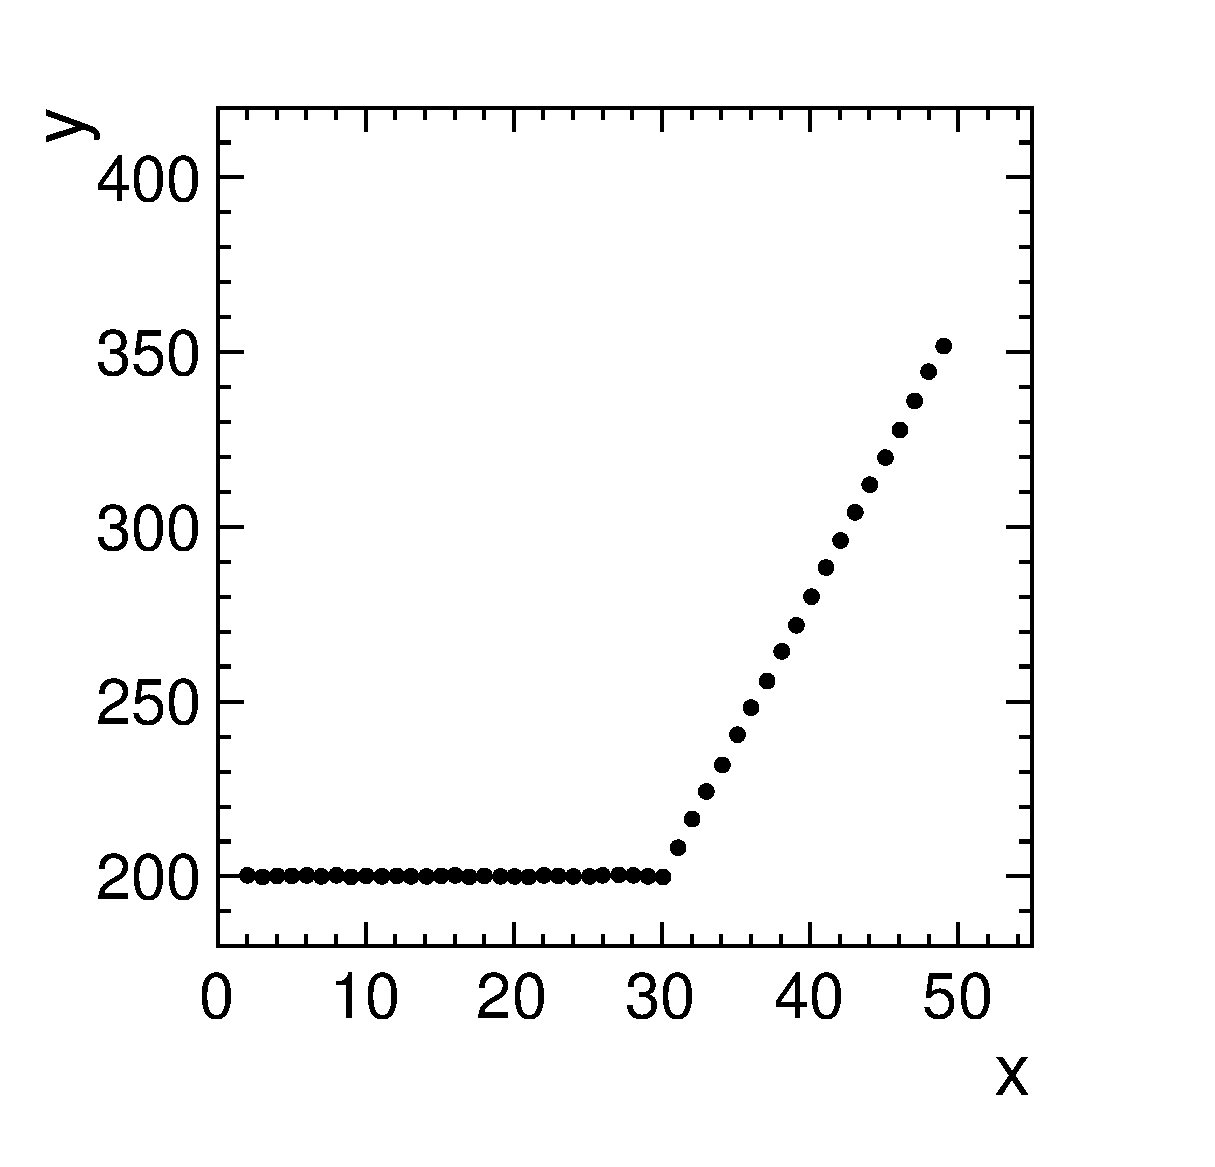
\includegraphics[width=50mm]{fig/hmap_kink_chi2.eps}
    \end{center}
    \caption{hit map like a Kaon track}
    \label{hmap3}
  \end{minipage}
  \begin{minipage}{0.5\hsize}
    \begin{center}
      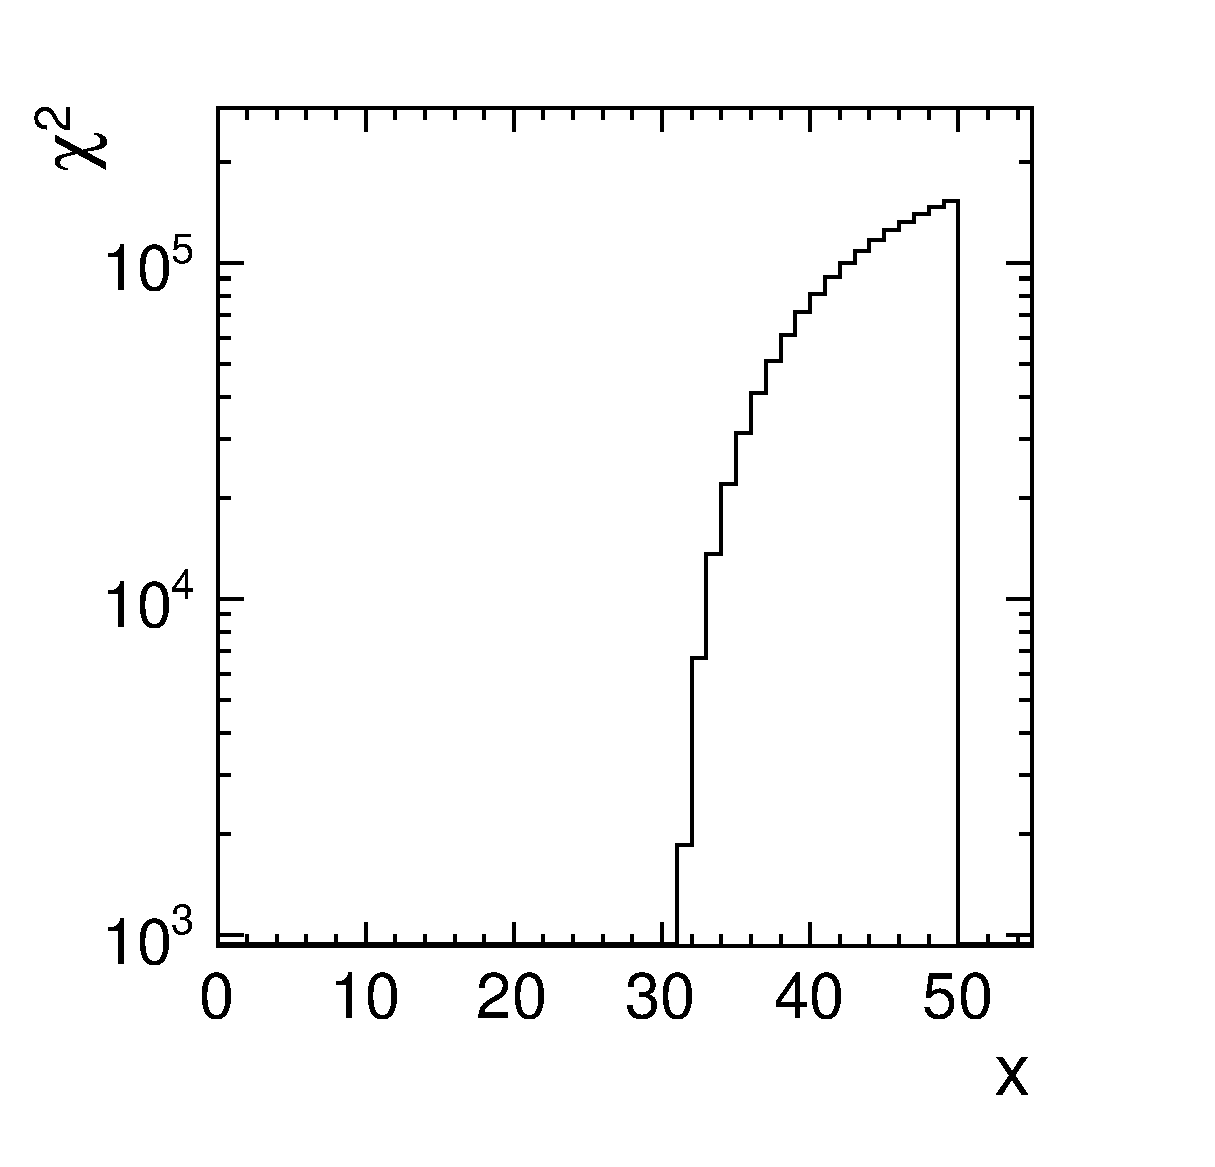
\includegraphics[width=50mm]{fig/chi2_kink_chi2.eps}
    \end{center}
    \caption{range vs $\chi^{2}$ distribution}
    \label{xvschi}
  \end{minipage}
\end{figure}


\subsubsection{BS method}
In the $\chi^{2}$ method , we can't find Kaon stopped point in the case of backward decay.
Then , we find Kaon stopped point using BS method.\\ 
BS method is concept that the Kaon stopped point defined as lightmost channel in the case of backward decay.
we descript below how the track defined as backward decay.
$N_{1}$ is defined as Number of cluster hits found by the clustering.
Stopped point finding is started from minimum channel.
We search for the closet timing hit in next channel from current channel hit. 
Then , we repeat this procedure until maximum channel and count the number of selected hit information($N_{2}$).
In the case of backward decay , $N_{1}$ is larger than $N{2}$.
So , we set reasonable threhold of the difference between $N_{1}$ and $N{2}$ , and if the $N_{1}>N_{2}$ is over the threshold , the track is defined as backward decay.
In the case of backward decay , we defined charge maximum point around the maximum channel as the stopped point. 

\begin{figure}[!htb]
  \begin{center}
    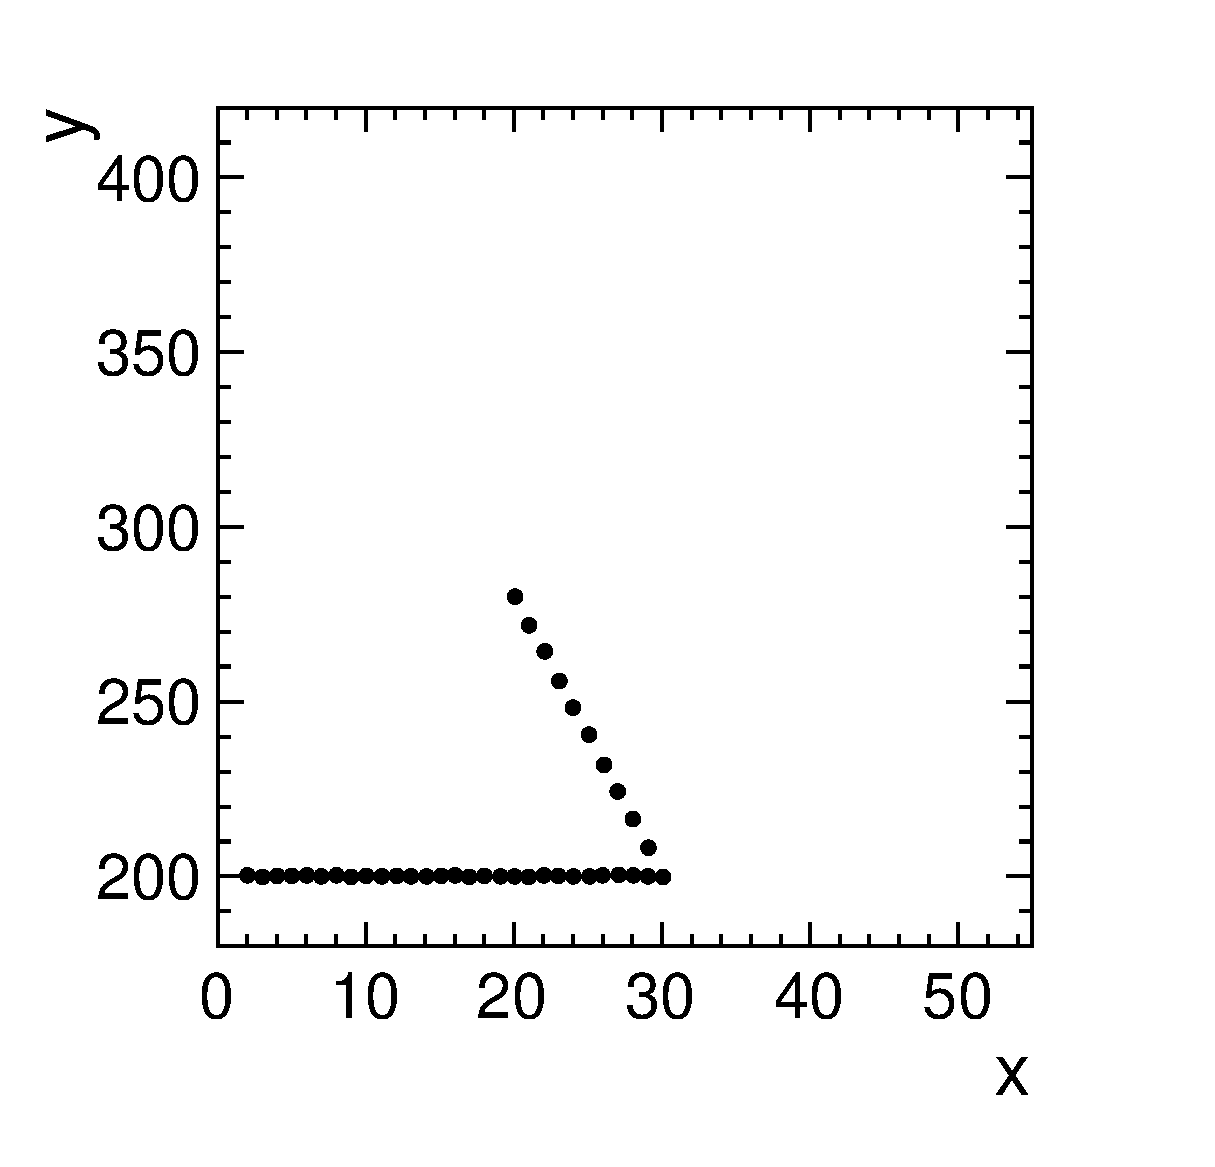
\includegraphics[width=50mm]{fig/hmap_kink_BS.eps}
  \end{center}
  \caption{hit map like a Kaon track}
  \label{hmap_BS}
\end{figure}





%%%%%%%%%%%%%%%%%%%%%%%%%%%%%%%%%%%%%%%%%%%%%%%%%%
%\section{Liquid Argon Purity}
%%%%%%%%%%%%%%%%%%%%%%%%%%%%%%%%%%%%%%%%%%%%%%%%%%
%%%%%%%%%%%%%%%%%%%%%%%%%%%%%%%%%%%%%%%%%%%%%%%%%%
\section{Liquid Argon Purity}
%%%%%%%%%%%%%%%%%%%%%%%%%%%%%%%%%%%%%%%%%%%%%%%%%%

Attenuation of the drift electron depends on purity of LAr since electronegative impurities capture it \cite{purity}. 
Thus we need to apply correction to TPC signal charge depends on the drift time.
We use cosmic ray sample triggered by inner PMT at off-beam timing for measuring the LAr purity, and use this to correct the beam data.
Figure~\ref{fig:CosmicEvent} shows an event display of typical cosmic muon event across TPC channels.
The attenuation of readout charge depending on drift time is clearly seen in the right plot. 
Readout charge in an event cannot be fitted by exponential because energy deposition follows Landau distribution and charge readout is affected by electric field distortion which is described latter in section~\ref{sec:Efield}.


%\begin{itemize}
%\item Plot: Typical Lifetime Fit  (Naganoma)
%\item Plot: Lifetime vs Time  (Naganoma)
%\end{itemize}

\begin{figure}[htbp]
 \begin{center}
  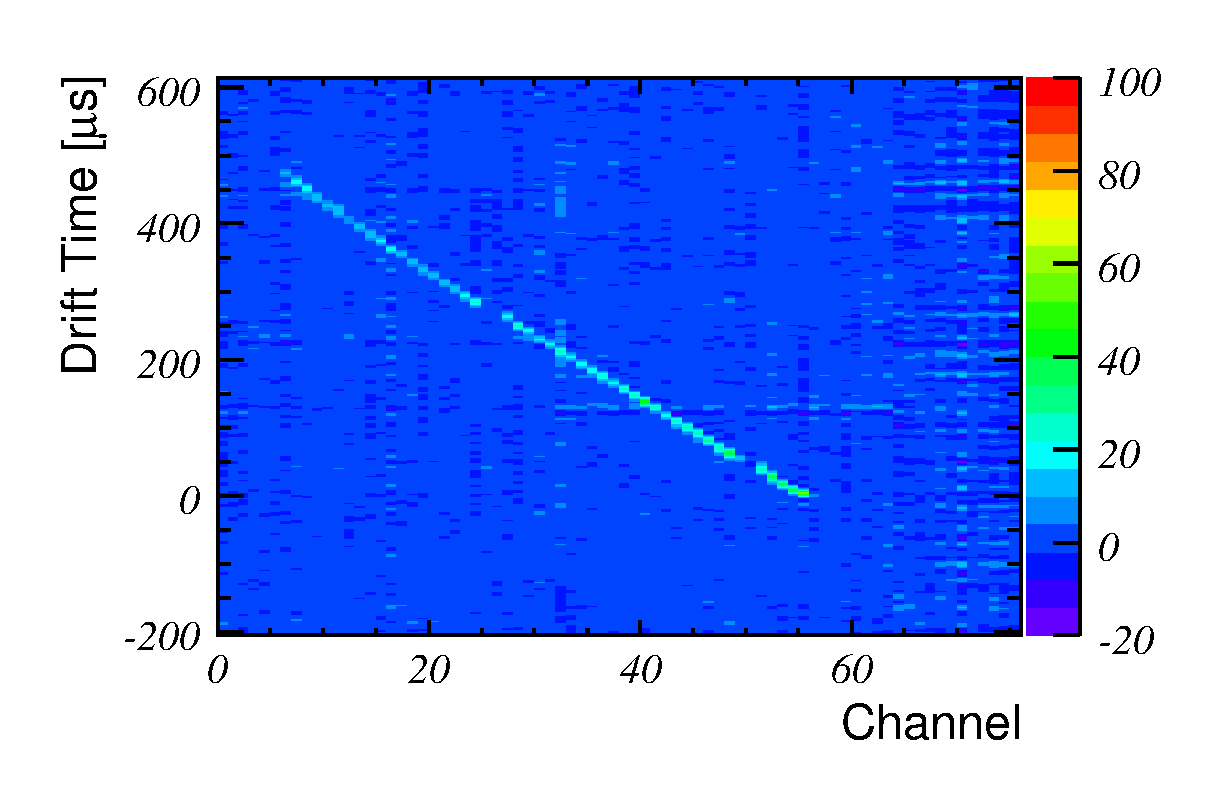
\includegraphics[width=60mm]{fig/cosmic68_ev258_display.eps}
  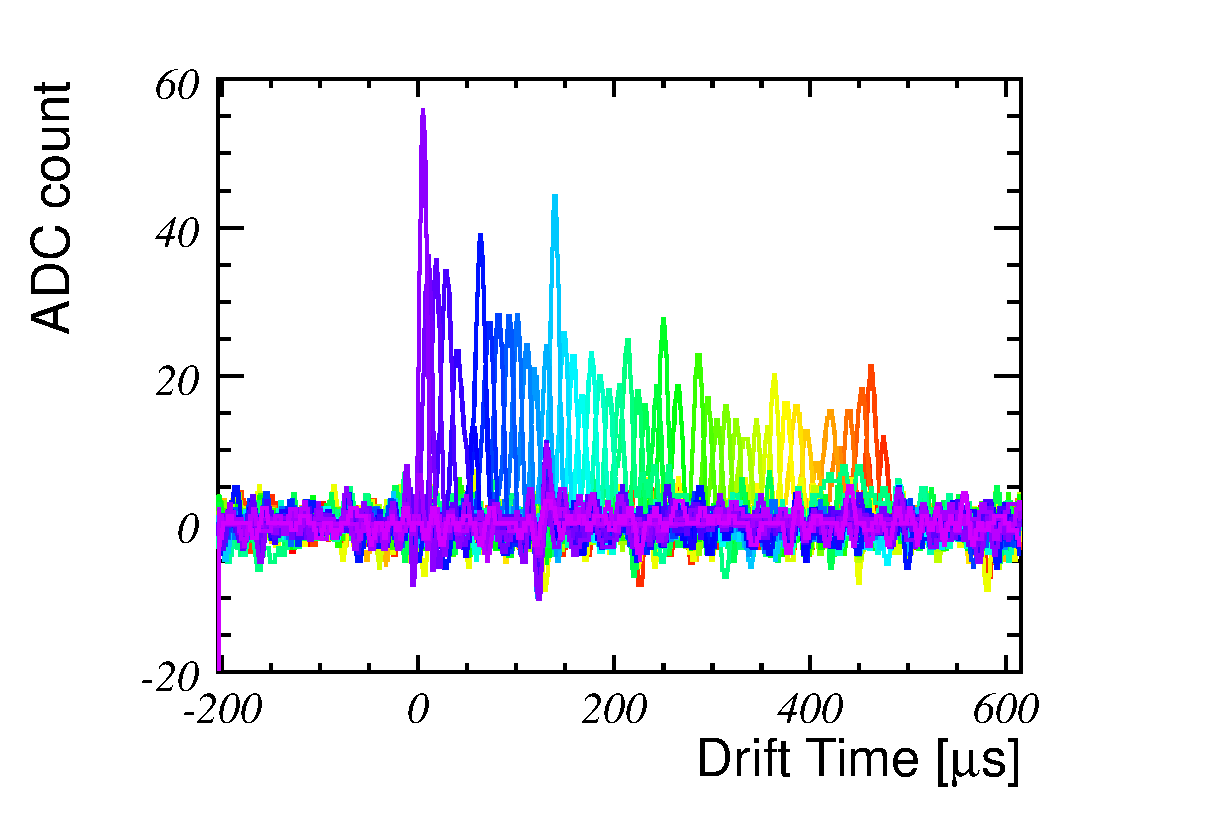
\includegraphics[width=60mm]{fig/cosmic68_ev258.eps}
 \end{center}
 \caption{Left: Typical cosmic muon event across TPC channels. Right: Charge deposit as a function of drift time. Colors correspond to different TPC channels.}
 \label{fig:CosmicEvent}
\end{figure}

We select cosmic ray event with more than 20 TPC channels which corresponds to zenith angle of more than $27^\circ$ and consistent with straight line by $\chi^2$ fit. 
Readout charge is corrected for field distortion and projected to beam direction to correct injection angle.
We fit readout charge by Landau function in each drift time bin to estimate average charge deposit. 
Figure~\ref{fig:tauExample} shows example of the average readout charge as a function of drift time which is fitted by exponential to obtain drift electron lifetime. 
Realistic Monte Carlo simulation shows about 13\% (TBU) smaller lifetime estimation due to noise, field distortion, and FFT effects. 
We correct output lifetime from these effects.
Figure~\ref{fig:CosmicPurity} shows an drift electron lifetime as a function of duration after initial LAr filling.
Drift electron lifetime was 600 $\mu$s at 60 hours, and 400 $\mu$s after 150 hours.
%Initial purity looks good, but the purity was slowly degrading while data taking period.
The degradation is possibly due to impurity from micro leak or out-gassing penetrating faster than purification by gas recirculation.
But we kept enough drift electron lifetime during data taking period.

\begin{figure}[htbp]
 \begin{center}
  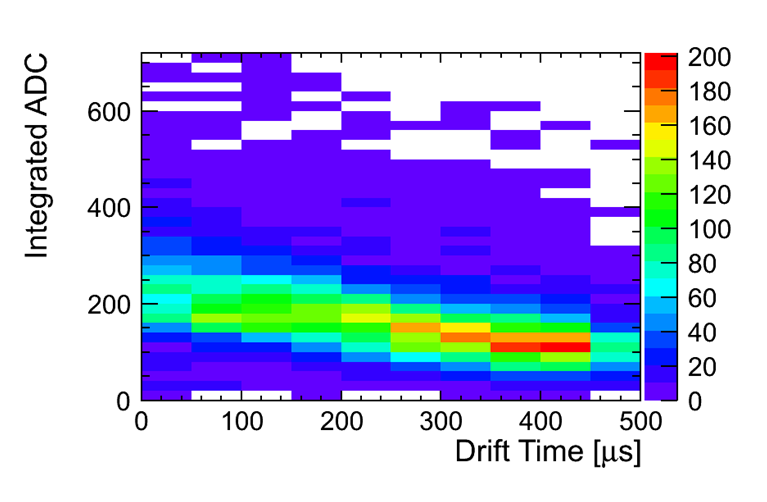
\includegraphics[width=60mm]{fig/chargeDep.eps}
  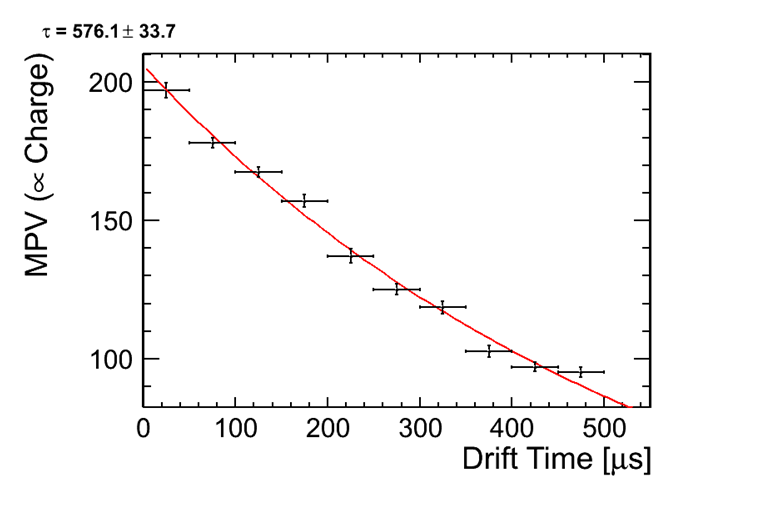
\includegraphics[width=60mm]{fig/tauExample.eps}
 \end{center}
 \caption{TBU. Left: Readout charge as a function of drift time. Readout charge in each drift time bin is fitted by landau function. Right: Average charge readout as a function of drift time which is fitted by exponential to estimate drift electron lifetime.}
 \label{fig:tauExample}
\end{figure}


\begin{figure}[htbp]
 \begin{center}
  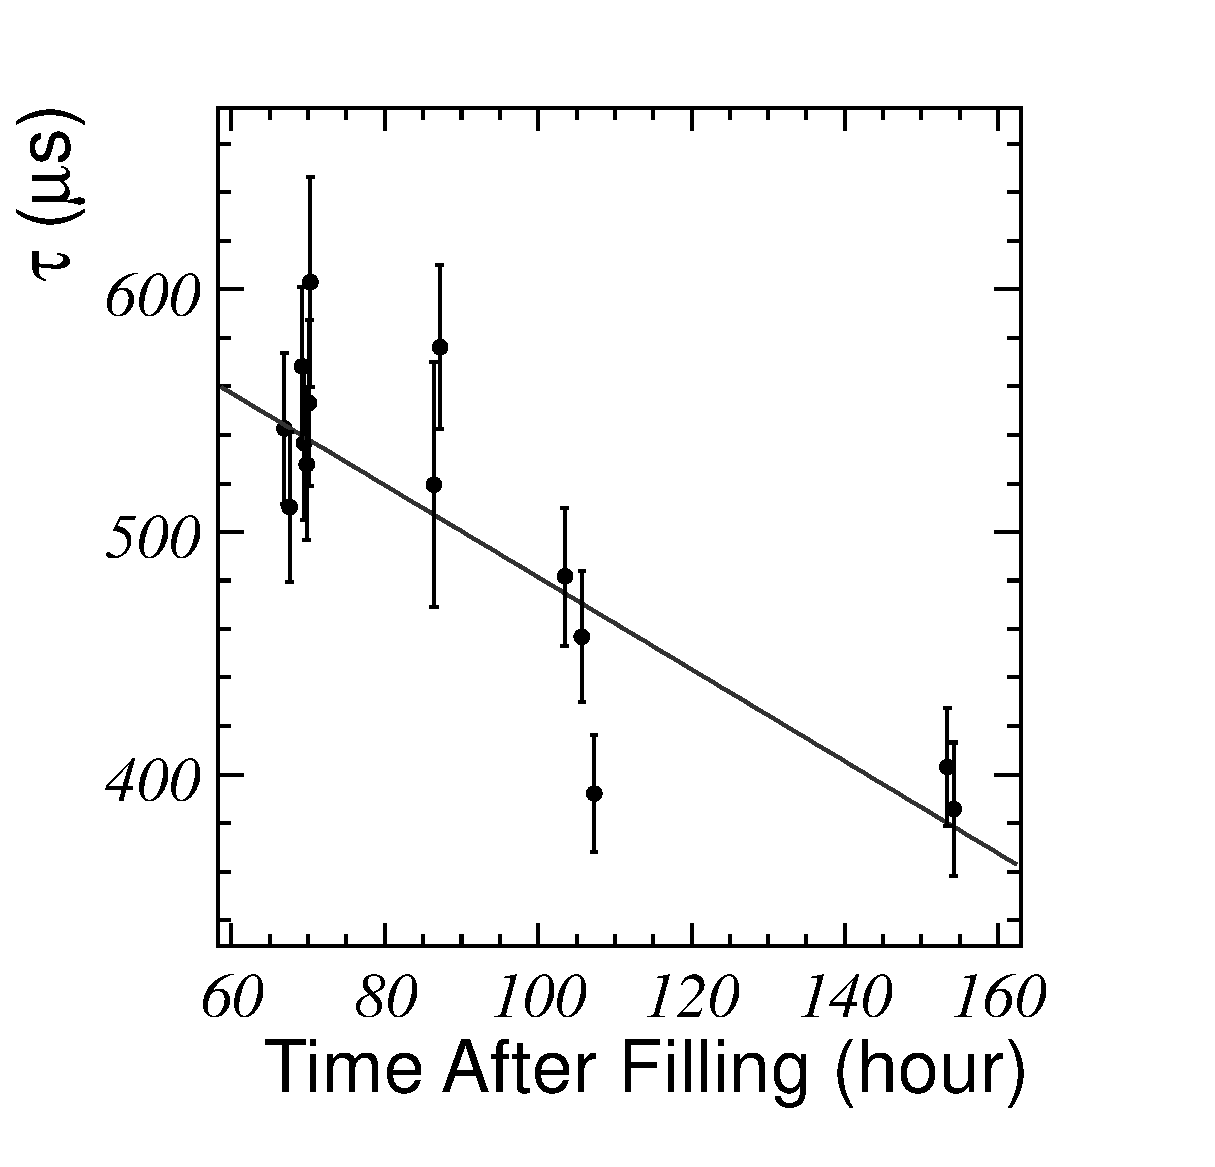
\includegraphics[width=60mm]{fig/tauHistory.eps}
 \end{center}
 \caption{TBU. Drift electron lifetime as a function of duration after initial LAr filling. The lifetime is used to correct the beam data.}
 \label{fig:CosmicPurity}
\end{figure}


%%%%%%%%%%%%%%%%%%%%%%%%%%%%%%%%%%%%%%%%%%%%%%%%%%
%\section{Event Simulation}
%%%%%%%%%%%%%%%%%%%%%%%%%%%%%%%%%%%%%%%%%%%%%%%%%%
%%%%%%%%%%%%%%%%%%%%%%%%%%%%%%%%%%%%%%%%%%%%%%%%%%
\section{Event Simulation}
%%%%%%%%%%%%%%%%%%%%%%%%%%%%%%%%%%%%%%%%%%%%%%%%%%
\subsection{Geant3, recombination, drift velocity}

We use GEANT3 for simulating energy deposition of beam particles and
their daughters. Readout pitch is 1 cm, 

we set the maximum step of Geant to 0.5 mm
which is enough smaller than the readout pitch of 1 cm.

It means charge deposition in one strip is typically 
simulated with 20 GEANT steps.

We set energy cut-off for soft electron/photon emission to
10 keV which is minimum possible energy can be set in GEANT3.
This cut-off is very important for  ionization electron recombination.

Recombination of electron and Argon ion depends on
the electric field and $dE/dx$. We use a measurement in Ref.\cite{658352}.
\begin{equation}
Q = A \frac{Q_0}{1 + k dE/dx}, A = 0.800, k = 0.486
\end{equation}

Velocity of the drift electron depends on the liquid Argon temperature
and the electric field. We use a measurement in Ref \cite{649233}.


\begin{verbatim}
 *     Special TPAR for TMED   3   Liquid_argon                                                    *
 *  CUTGAM= 10.00 keV  CUTELE= 10.00 keV  CUTNEU= 10.00 MeV  CUTHAD= 10.00 MeV  CUTMUO= 10.00 MeV  *
 *  BCUTE = 10.00 keV  BCUTM = 10.00 keV  DCUTE = 10.00 keV  DCUTM = 10.00 keV  PPCUTM= 10.00 MeV  *
 *  IPAIR=  1.  ICOMP=  1.  IPHOT=  1.  IPFIS=  0.  IDRAY=  1.  IANNI=  1.  IBREM=  1.  IHADR=  4. *
 *  IMUNU=  1.  IDCAY=  1.  ILOSS=  1.  IMULS=  1.  IRAYL=  0.  ILABS=  0.  ISYNC=  0.  ISTRA=  0. *
\end{verbatim}



\begin{itemize}
\item Plot: Geant Geometry, typical track (Tanaka)
\item Plot: recombination factor, drift velocity  (Tanaka)
\end{itemize}

\subsection{Electric Field}

Electric field of the TPC field cage
We have calculated the electric field using a 2D FEM (Finite Element Method) package \cite{Ref:FEMTET}.

This field map is used for simulating electron drift.


\begin{itemize}
\item Plot: 2D field map  (Tanaka)
\end{itemize}

\subsection{Drift Electron Diffusion}
\begin{itemize}
\item Plot: drift simulation  (Tanaka)
\end{itemize}

\subsection{Preamp Gain Calibration}
\begin{itemize}
\item Preamp gain vs channel number  (Naito)
\end{itemize}

\subsection{FFT Noise}
\begin{itemize}
\item Plot: simulated event  (Nagasaka)
\end{itemize}

\subsection{Cross Talk}
\begin{itemize}
\item Plot: signal waveform (proton stopped point + 1)  (A. Okamoto)
\item Plot: simulated event with and without cross talk (A. Okamoto)
\end{itemize}

\subsection{Signal and Noise Scale Tuning}
\begin{itemize}
\item Plot: Landau distribution after the tuning  (Tanaka)
\end{itemize}


%%%%%%%%%%%%%%%%%%%%%%%%%%%%%%%%%%%%%%%%%%%%%%%%%%
%\section{Data-MC Comparison}
%%%%%%%%%%%%%%%%%%%%%%%%%%%%%%%%%%%%%%%%%%%%%%%%%%
%%%%%%%%%%%%%%%%%%%%%%%%%%%%%%%%%%%%%%%%%%%%%%%%%%
\section{Data- MC Comparison}
%%%%%%%%%%%%%%%%%%%%%%%%%%%%%%%%%%%%%%%%%%%%%%%%%%
\subsection{Through-going Pion}
\begin{itemize}
\item Plot: Data-MC comparison  (Tanaka)
\end{itemize}

\subsection{Stopped Proton}
\begin{itemize}
\item Plot: Hit charge, cluster charge, stopped point  (A. Okamoto)
\item Plot: hit charge with different distance from SP   (A. Okamoto)
\item Plot: average hit charge vs different distance from SP   (A. Okamoto)
\end{itemize}

%\subsection{Recombination Factor}
\subsection{Recombination Factor}
%In this analysis, we use parameters of the Recombination factor in a measurement of Ref.\cite{658352}.
 Electron-ion recombination depends on the electric field and stopping power $dE/dx$. We study this factor using tagged proton beam. Recombination factor measurement using proton beam is relatively easy because of stability of proton. This is why we used proton beam for this study as a first step.\\
  Expression for recombination can be derived 

\begin{equation}
  Q = A\frac{Q_{0}}{1+(k/E)\times(dE/dx)\times(1/\rho)}
\end{equation}

where $Q_{0}$ is initial ionization charge, $E$ is electric field, $dE/dx$ is energy deposit per distance, $\rho$ is density of liquid Argon, A and k are fit parameters. This formula can be rearranged like below:

\begin{equation}
  \frac{Q_{0}}{Q} = \frac{1}{A}+\frac{(k/E)(dE/dx)(1/\rho)}{A}
\end{equation}

The ratio of $Q_{0}/Q$ depends on stopping power $dE/dx$, so we determined fit parameter A and k using proton data and Monte Carlo simulation. In this analysis, we need $Q$, $Q_{0}$ and $dE/dx$ channel by channel. First, electric field $E$ was 200 V/cm in our test. Second, $Q$ is integrated charge in an anode readout channel. Third, $Q_{0}$ is integrated charge without recombination factor in an anode readout channel. And then, $dE/dx$ per an anode channel is determined with truth information of Monte Carlo simulation. Figure \ref{fadcDist1}, \ref{fadcDistMC}, \ref{fadcDistdEdx} show $Q$, $Q_{0}$, $dE/dx$ as a function of distance from stopped channel between 1 to 14 channel. $Q$ is obtained from data, $Q_{0}$ and $dE/dx$ are obtained from Monte Carlo simulation.
In many case, integrated charge in stopped channel are more affected by noise from next channel. This is the reason why we don't use information from stopped channel in this analysis. 

%ch by ch data distribution
\begin{figure}[!htb]
  \centering
  \centering
  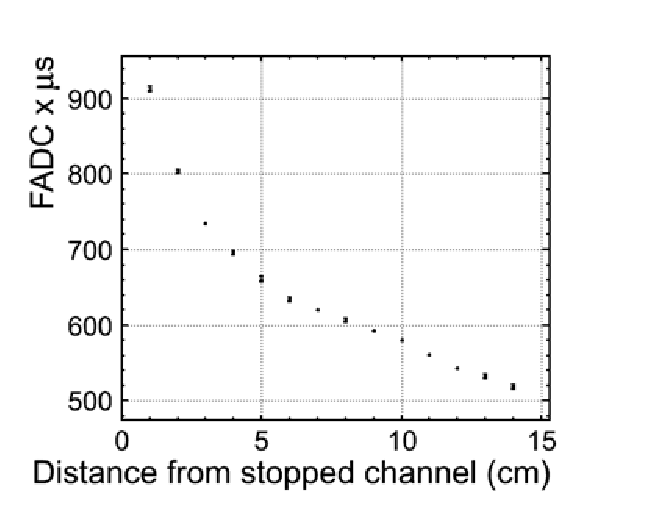
\includegraphics[width=11cm,clip]{./fig/q.eps}
%  \includegraphics[width=11cm,clip]{./fig/Data_FADCdistChbyCh.eps}
  \caption{DATA:Integrated Flash ADC counts from stopped channel -1}
  \label{fadcDist1}
\end{figure}
\pagebreak
\pagebreak

The result of this study is shown in Fig\ref{result}. Vertical axis is $Q_{0}/Q$, and horizontal axis is $dE/dx$ in this figure, this plot is fitted by Birks law.
As a result, we got fitting parameter\\
\begin{eqnarray}
%  \center
 \nonumber  A =& 0.782\pm0.009\\
   k =& 0.0467\pm0.0009 [kV(g/cm^{2})/cm/MeV]
\end{eqnarray}

We checked Birks law in the range 4 $MeV/(g/cm^2)$ $\leqq dE/dx \leqq$ 12 $MeV/cm^2$ and the result is consistent with ICARUS experiment's one\cite{658352} in -- sigma.

%ch by ch MC distribution
\begin{figure}[!htb]
  \centering
  \centering
  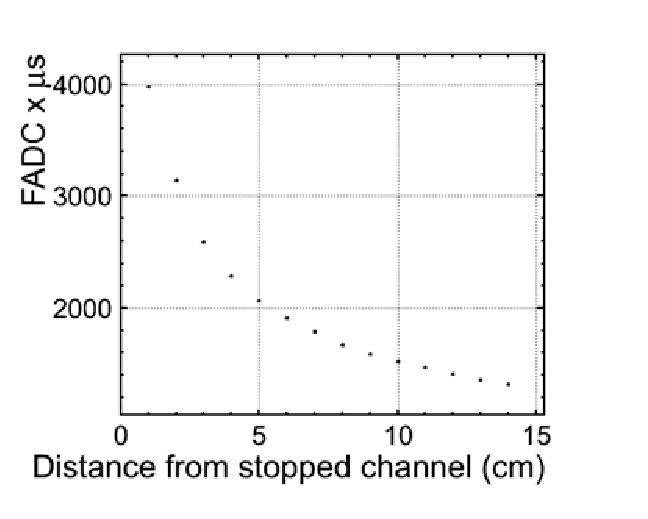
\includegraphics[width=11cm,clip]{./fig/q_0.eps}
%  \includegraphics[width=11cm,clip]{./fig/MC_FADCdistChbyCh.eps}
%  \caption{MC:Distribution of Flash ADC counts ch by ch
  \caption{MC without recombination:Integrated Flash ADC counts from stopped channel -1}
  \label{fadcDistMC}
\end{figure}

%ch by ch dE/dx distribution
\begin{figure}[!htb]
  \centering
  \centering
  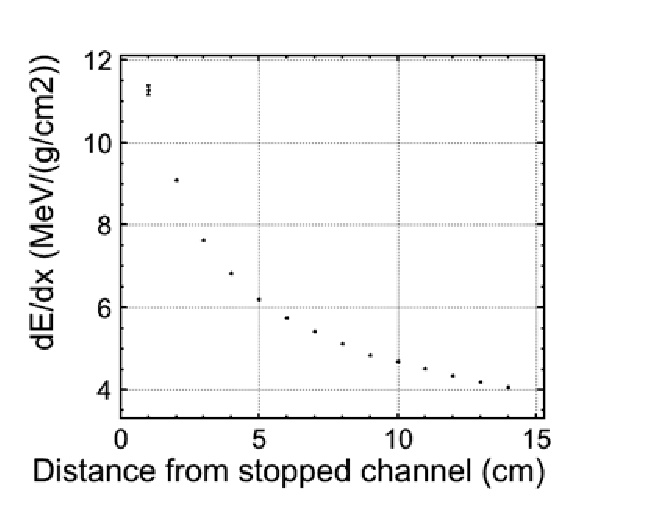
\includegraphics[width=11cm,clip]{./fig/dedx.eps}
%  \caption{Distribution of dE/dx ch by ch}
  \caption{dE/dx from stopped channel -1}
  \label{fadcDistdEdx}
\end{figure}

%result
\begin{figure}[!htb]
  \centering
  \centering
  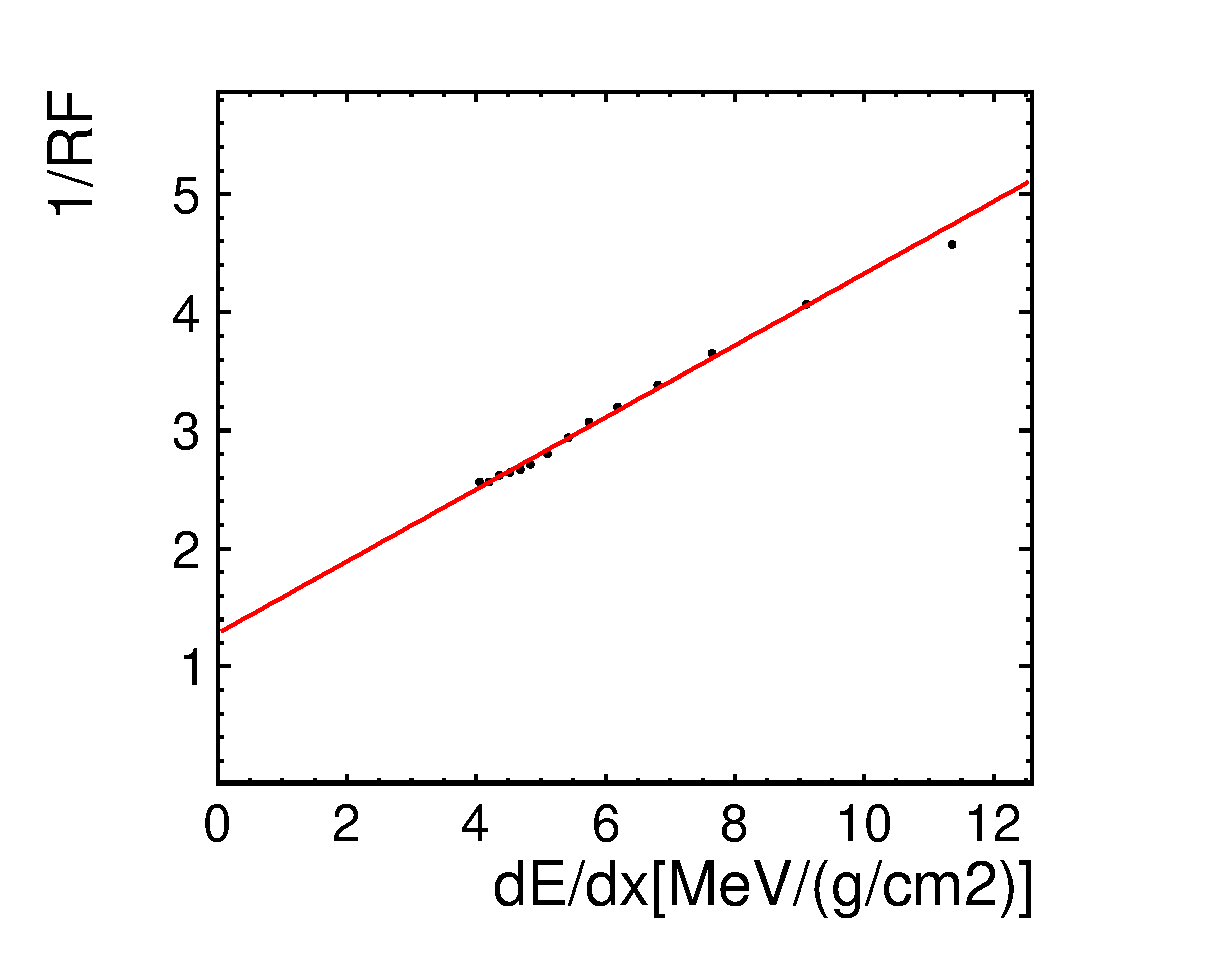
\includegraphics[width=11cm,clip]{./fig/result.eps}
  \caption{1/RF VS dE/dx: fitted by Birks law}
  \label{result}
\end{figure}


%\subsection{Stopped Kaon}
\subsection{Stopped Kaon}
In this section, we compare some quantities of data and MC simulation that K stops in the liquid argon detector and we can find stopped point.
Figure \ref{KsomeQuantities} shows Data and MC comparison for signal hit charge, signal width, decay point and total particle charge distribution.
Data of signal charge and signal width are consistent with MC one in error by less than two $\%$ and data of cluster charge and primary charge are consistent with  MC one in error by less than five $\%$.

Figure \ref{cq27_hough} shows signal hit charge distribution of restricted channel 27. 
As shown in figure \ref{cq27_hough}, signal charge have two peaks at 300 and 500 ADCus.
Because two peaks has correlation of $\Delta$TOF, possible assumption of the cause is that beam line were bipolarrized and the beam didn't pass in the center of the detector.
So, we use only the event that signal charge of restricted channel 27 is less than 350.
Figure \ref{RangeVsHit_hough} shows signal hit charge distribution in different distance from the stopped point.

\begin{figure}[htbp]
  \begin{center}
    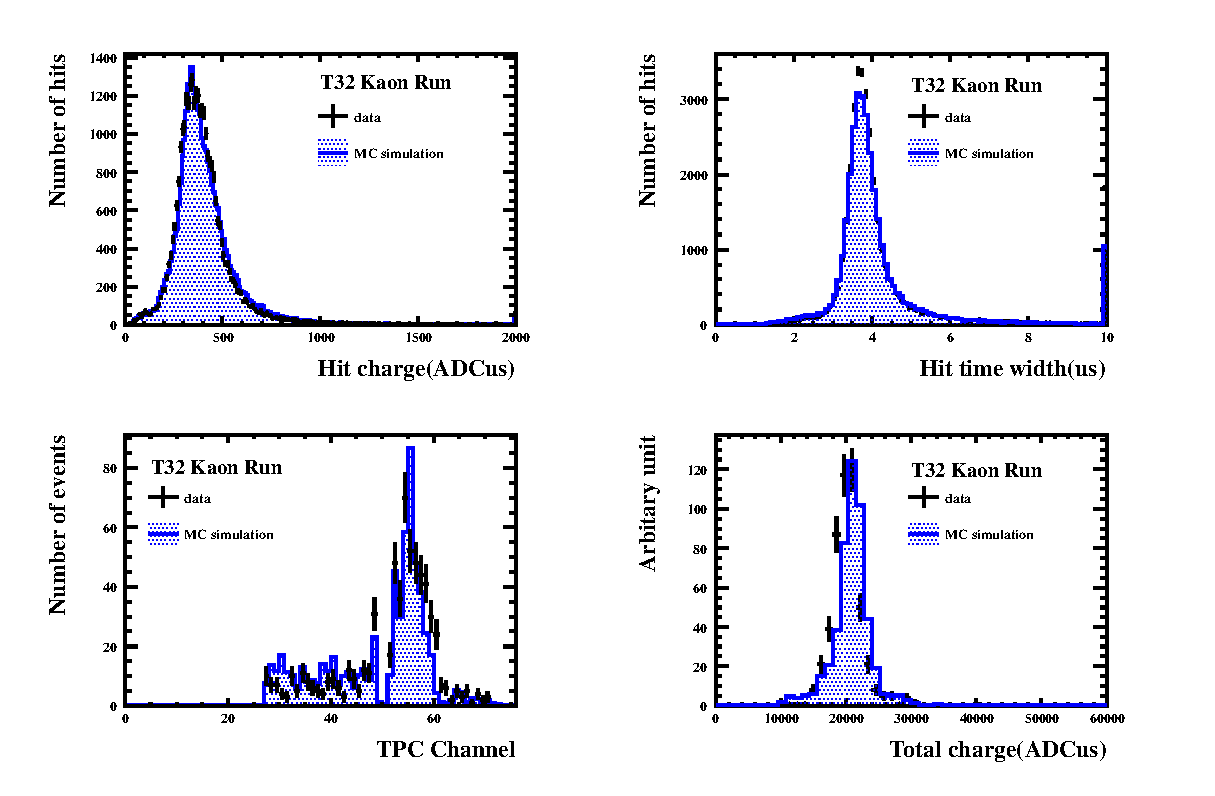
\includegraphics[width=70mm]{fig/cHit4_hough.eps}
  \end{center}    
    \caption{Data-MC comparison for hit charge, hit sigma, cluster charge, primary particle charge}
    \label{KsomeQuantities}
\end{figure}



\begin{figure}[!htb]
  \begin{center}
    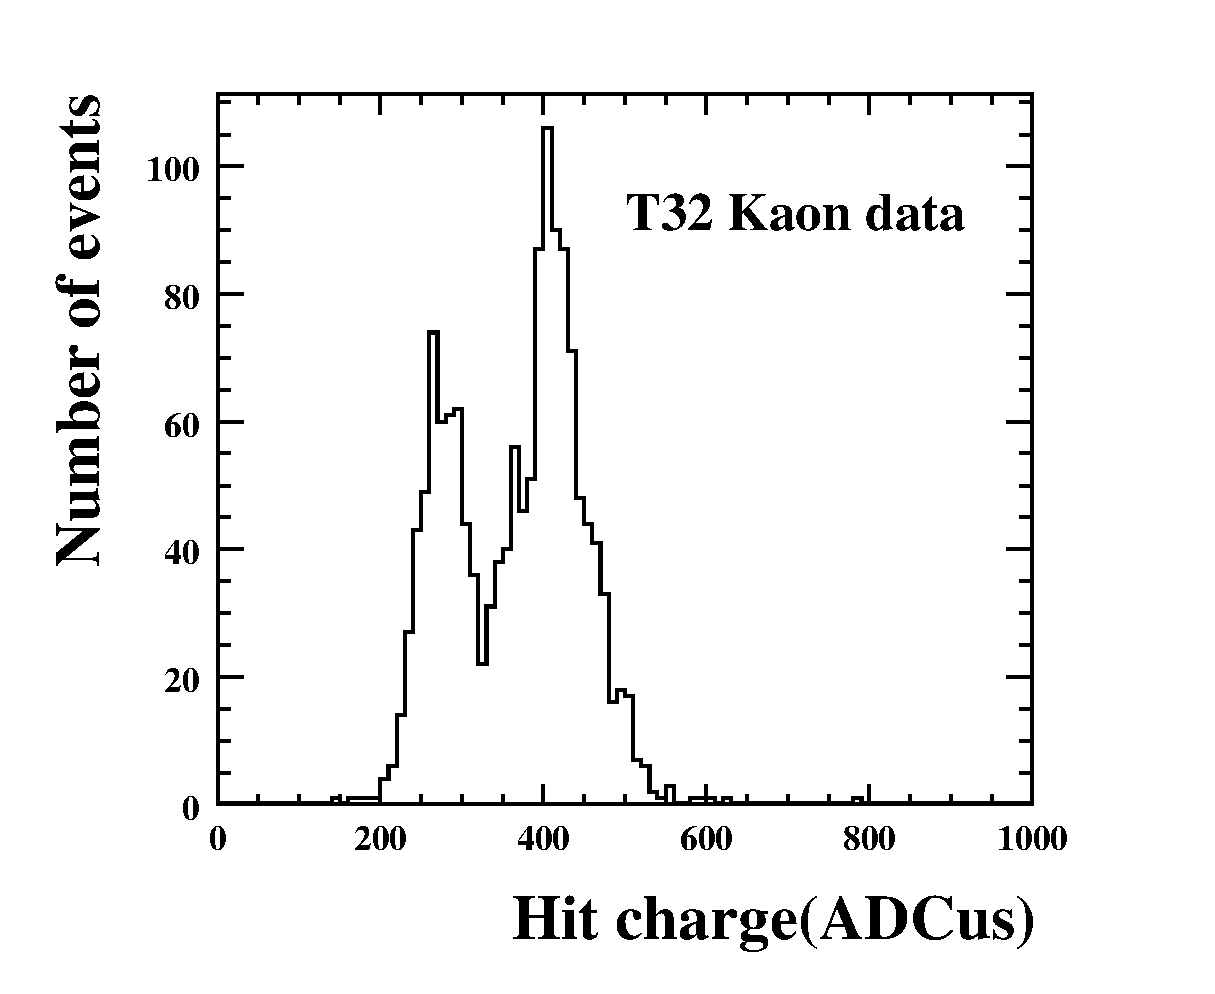
\includegraphics[width=70mm]{fig/ch27distribution.eps}
  \end{center}
  \label{cq27_hough}
  \caption{Hit charge in channel 27}
\end{figure}

\begin{figure}[!htb]
  \begin{center}
    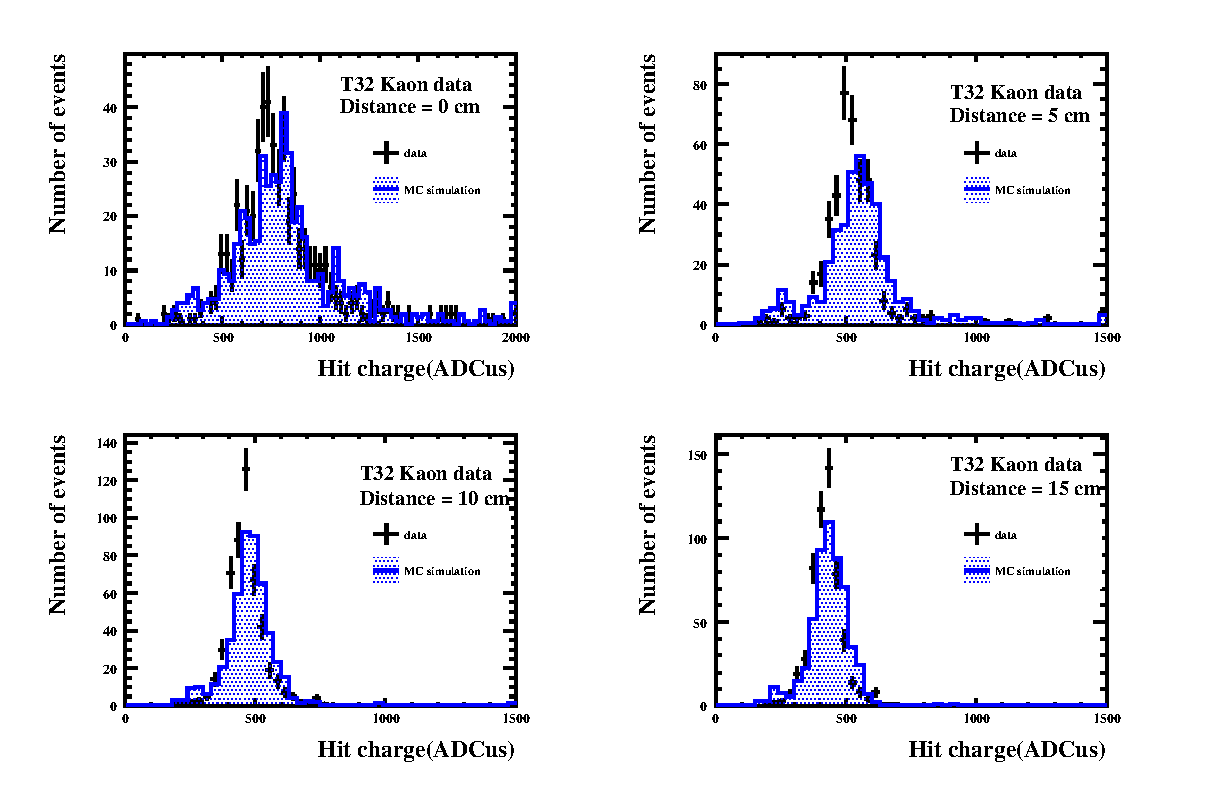
\includegraphics[width=100mm]{fig/RangeVsHit4_wcut_hough.eps}
  \end{center}
  \caption{Data-MC comparison for hit charge distribution in different distance from the stopped point(top left:decay point,top light:decay point-5cm,bottom left:decay point-10cm,decay point-15cm)}
  \label{RangeVsHit_hough}
\end{figure}

As shown in figure \ref{RangeVsHit_hough}, data is consistent with MC one.
Figure \ref{RangeVsHitRatio_hough} shows data/MC ratio of signal hit charge distribution in different distance from the stopped point.
Data of signal charge in different distance from stopped point are consistent with MC one with in 5$\%$.

\begin{figure}[htb]
  \begin{center}
    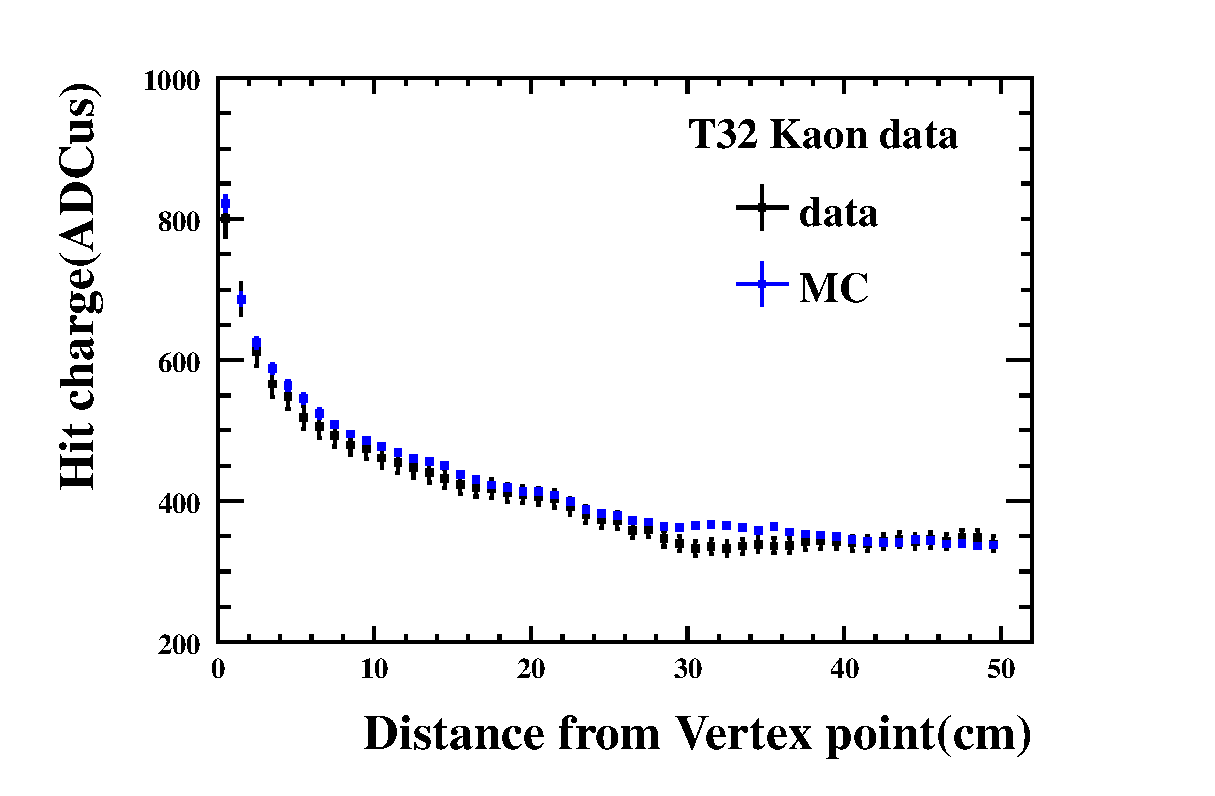
\includegraphics[width=70mm]{fig/RangeVsHitfabs_wcut_hough.eps}
  \end{center}
  \caption{Data-MC comparison for hit charge distribution in different distance from the stopped point}
  \label{RangeVsHitfabs_hough}
\end{figure}

\begin{figure}[htb]
  \begin{center}
    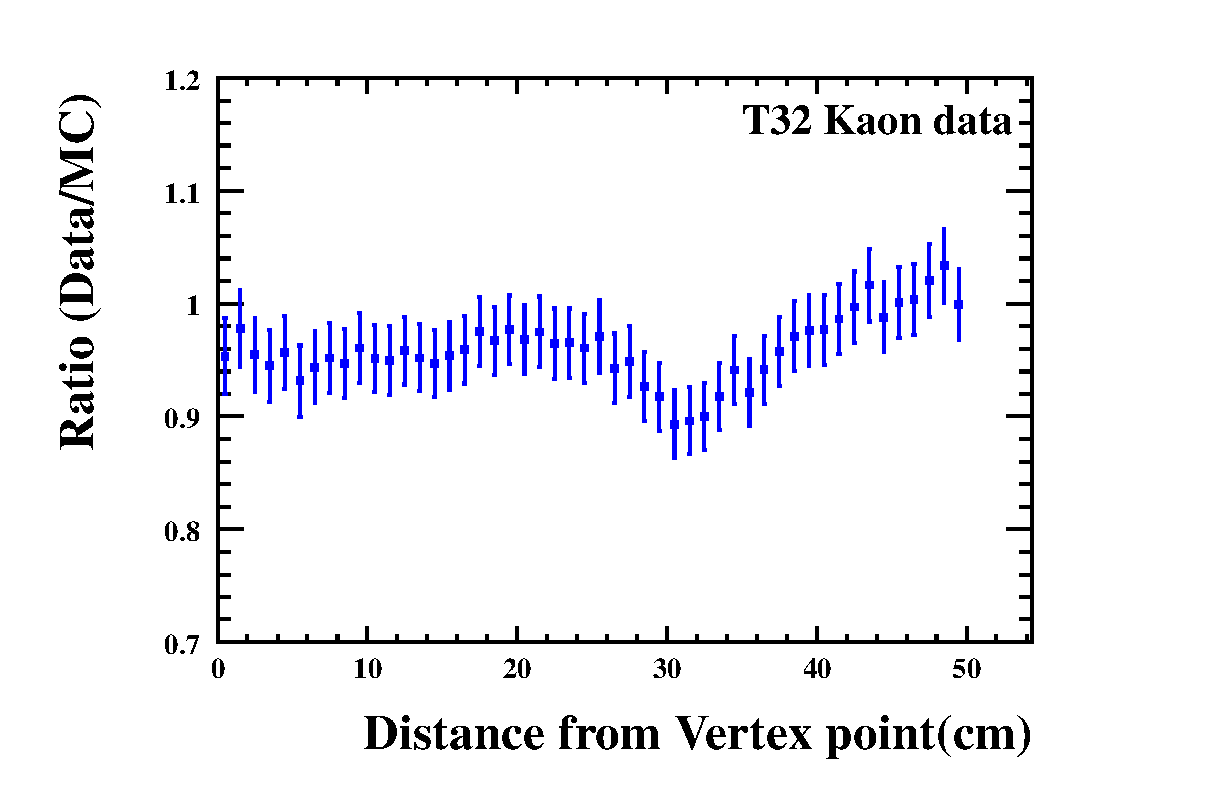
\includegraphics[width=70mm]{fig/RangeVsHitRatio_wcut_hough.eps}
  \end{center}
  \caption{Data/MC ratio for hit charge distribution in different distance from the stopped point}
  \label{RangeVsHitRatio_hough}
\end{figure}






%%%%%%%%%%%%%%%%%%%%%%%%%%%%%%%%%%%%%%%%%%%%%%%%%%
%\section{Summary}
%%%%%%%%%%%%%%%%%%%%%%%%%%%%%%%%%%%%%%%%%%%%%%%%%%
\section{Summary}
\begin{itemize}
\item We have constructed 250L LArTPC
\item Collected high purity Pion, Kaon, and proton sample
\item Establish Kaon stopped point finding algorithm
\item Develop realistic detector simulation
\item Good understanding of Pion Landau distribution
\item Good understanding of Proton and Kaon dE/dx
\item Measurement of recombination using pi, K, and proton
\end{itemize}


%% The Appendices part is started with the command \appendix;
%% appendix sections are then done as normal sections
%% \appendix

%% \section{}
%% \label{}

%% References
%%
%% Following citation commands can be used in the body text:
%% Usage of \cite is as follows:
%%   \cite{key}         ==>>  [#]
%%   \cite[chap. 2]{key} ==>> [#, chap. 2]
%%

%% References with bibTeX database:

\bibliographystyle{elsarticle-num}
\bibliography{<your-bib-database>}

%% Authors are advised to submit their bibtex database files. They are
%% requested to list a bibtex style file in the manuscript if they do
%% not want to use elsarticle-num.bst.

%% References without bibTeX database:

\begin{thebibliography}{00}

%% \bibitem must have the following form:
%%   \bibitem{key}...
%%

% \bibitem{}
%\cite{Araoka:2011pw}
\bibitem{Araoka:2011pw}
  O.~Araoka {\it et al.},
  %``A tagged low-momentum kaon test-beam exposure with a 250L LAr TPC (J-PARC
  %T32),''
  J.\ Phys.\ Conf.\ Ser.\  {\bf 308}, 012008 (2011)
  [arXiv:1105.5818 [physics.ins-det]].
  %%CITATION = 00462,308,012008;%%

\bibitem{Mihara:2004ft}
S.~Mihara [MEG Collaboration],
%``R&D work on a liquid-xenon photon detector for MEG experiment at PSI,''
Nucl.\ Instrum.\ Meth.\ A {\bf 518}, 45 (2004).
%%CITATION = NUIMA,A518,45;%%

%\cite{658352}
\bibitem{658352} 
  S.~Amoruso {\it et al.} [ICARUS Collaboration],
  %``Study of electron recombination in liquid argon with the ICARUS TPC,''
  Nucl.\ Instrum.\ Meth.\ A\ {\bf 523}, 275  (2004).
  %%CITATION = NUIMA,A523,275;%%

%\cite{649233}
\bibitem{649233} 
  S.~Amoruso, M.~Antonello, P.~Aprili, F.~Arneodo, A.~Badertscher, B.~Baibusinov, M.~Baldo-Ceolin and G.~Battistoni {\it et al.},
  %``Analysis of the liquid argon purity in the ICARUS T600 TPC,''
  Nucl.\ Instrum.\ Meth.\ A\ {\bf 516}, 68  (2004).
  %%CITATION = NUIMA,A516,68;%%

\bibitem{purity}
  A.~Bettini {\it et al.}, Nucl.\ Instrum.\ Meth.\ A\ {\bf 305}, 1991  (177).

\bibitem{3069654}
  P.V.C Hough 'Method and means for recognizing complex patterns',United States Patent Office 3069654(1962) 

\end{thebibliography}


\end{document}

%%
%% End of file `elsarticle-template-num.tex'.
